\documentclass[12pt]{amsart}

\usepackage{amstext,amsfonts,amssymb,amscd,amsbsy,amsmath,verbatim}
\usepackage{diagrams}
\usepackage[alphabetic,backrefs,lite]{amsrefs} %bibliography
\usepackage{ifthen, fullpage}
\usepackage{extarrows}
\usepackage{color,tikz,multirow}
\usepackage{amsthm}
\usepackage{latexsym}
\usepackage[all]{xy}
\usepackage{enumerate}



\newtheorem{lemma}{Lemma}[section]
\newtheorem{theorem}[lemma]{Theorem}
\newtheorem{propo}[lemma]{Proposition}
\newtheorem{prop}[lemma]{Proposition}
\newtheorem{cor}[lemma]{Corollary}
\newtheorem{conj}[lemma]{Conjecture}
\newtheorem{claim}[lemma]{Claim}
\newtheorem{claim*}{Claim}
\newtheorem{thm}[lemma]{Theorem}
\newtheorem{notation}[lemma]{Notation}

\theoremstyle{definition}


\theoremstyle{remark}
\newtheorem{defn}[lemma]{Definition}
\newtheorem{example}[lemma]{Example}
\newtheorem{remark}[lemma]{Remark}
\newtheorem{question}[lemma]{Question}

% Commands

\newcommand{\isom}{\cong}
\newcommand{\m}{\mathfrak m}
\newcommand{\lideal}{\langle}
\newcommand{\rideal}{\rangle}
\newcommand{\initial}{\operatorname{in}}
\newcommand{\Hilb}{\operatorname{Hilb}}
\newcommand{\hilb}{\operatorname{hilb}}
\newcommand{\Spec}{\operatorname{Spec}}
\newcommand{\im}{\operatorname{im}}
\newcommand{\NS}{\operatorname{NS}}
\newcommand{\Frac}{\operatorname{Frac}}
\newcommand{\ch}{\operatorname{char}}
\newcommand{\Proj}{\operatorname{Proj}}
\newcommand{\id}{\operatorname{id}}
\newcommand{\Div}{\operatorname{Div}}
\newcommand{\tr}{\operatorname{tr}}
\newcommand{\Tr}{\operatorname{Tr}}
\newcommand{\supp}{\operatorname{supp}}
\newcommand{\Gal}{\operatorname{Gal}}
\newcommand{\Pic}{\operatorname{Pic}}
\newcommand{\QQbar}{{\overline{\mathbb Q}}}
\newcommand{\Br}{\operatorname{Br}}
\newcommand{\Bl}{\operatorname{Bl}}
\newcommand{\Cox}{\operatorname{Cox}}
\newcommand{\Tor}{\operatorname{Tor}}
\newcommand{\Tot}{\operatorname{Tot}}
\newcommand{\diam}{\operatorname{diam}}
\newcommand{\Hom}{\operatorname{Hom}} %done
\newcommand{\Ext}{\operatorname{Ext}} %done
\newcommand{\sheafHom}{\mathcal{H}om}
\newcommand{\Gr}{\operatorname{Gr}}
\newcommand{\Osh}{{\mathcal O}}
\newcommand{\kk}{\Bbbk}
\newcommand{\coker}{\operatorname{coker}}
\newcommand{\rank}{\operatorname{rank}}
\newcommand{\pt}{\text{pt}}
\newcommand{\codim}{\operatorname{codim}}
\newcommand{\PP}{\mathbb{P}}
\renewcommand{\AA}{\mathbb{A}}
\newcommand{\GG}{\mathbb{G}}
\newcommand{\HH}{\mathrm{H}}
\newcommand{\KK}{\mathrm{K}}
\newcommand{\ZZ}{\mathbb{Z}}
\newcommand{\QQ}{\mathbb{Q}}
\newcommand{\UU}{\mathrm{U}}
\newcommand{\VV}{\mathrm{V}}
\newcommand{\WW}{\mathrm{W}}
\newcommand{\Wvb}{\mathrm{W}_{\text{vb}}}
\newcommand{\NN}{\mathbb{N}}
\newcommand{\CC}{\mathbb{C}}
\newcommand{\RR}{\mathbb{R}}
\newcommand{\cc}{c}
\newcommand{\dd}{d}
%\newcommand{\dd}{\mathbf{d}}
\newcommand{\bmin}{\mathbf{b}_{\text{min}}}
\newcommand{\bmax}{\mathbf{b}_{\text{max}}}
\newcommand{\uHH}{\underline{\mathsf{H}}}
\newcommand{\cO}{\mathcal{O}}
\newcommand{\cE}{\mathcal{E}}
\newcommand{\cF}{\mathcal{F}}
\newcommand{\cU}{\mathcal{U}}
\newcommand{\EE}{\mathbf{E}}
\newcommand{\bB}{\mathbf{B}}
\newcommand{\bG}{\mathbf{G}}
\newcommand{\bK}{\mathbf{K}}

\newcommand{\FF}{\mathbf{F}}
\newcommand{\Gbull}{\mathbf{G}}
\newcommand{\Kbull}{\mathbf{K}}
\newcommand{\Sym}{\operatorname{Sym}} %done  
\newcommand{\GL}{{GL}}
\newcommand{\Syz}{\operatorname{Syz}}
\newcommand{\pos}{\operatorname{pos}}

\newcommand{\defi}[1]{\textsf{#1}} % for defined terms



\newcommand{\zp}{\circ}
\newcommand{\nothing}{\emptyset}
\newcommand{\BQ}{\mathrm{B}}
\newcommand{\DD}{\mathrm{D}}
\newcommand{\w}{\widetilde}
\newcommand{\CQ}{\mathrm{C}}
\newcommand{\CvbQ}{\mathrm{C}_{\text{vb}}}
\newcommand{\BBQ}{\mathrm{B}}
\newcommand{\BBirr}{\underline{\mathrm{B}}^{\text{irr}}}
\newcommand{\CCQ}{\underline{\mathrm{C}}}
\newcommand{\Bmod}{\ensuremath{B_\text{mod}}}
\newcommand{\Bint}{\ensuremath{B_\text{int}}}
\newcommand{\Lotimes}{\overset{\mathrm{L}}{\otimes}}
\newcommand{\daniel}[1]{{\color{green} \sf $\clubsuit\clubsuit\clubsuit$ Daniel: [#1]}}
\newcommand{\mauricio}[1]{{\color{blue} \sf $\clubsuit\clubsuit\clubsuit$ Mauricio: [#1]}}
\newcommand{\david}[1]{{\color{red} \sf $\clubsuit\clubsuit\clubsuit$ David: [#1]}}

\renewcommand{\P}{{\mathbb P}}
\def\edim{\operatorname{edim}}
\def\reg{\operatorname{reg}}
\def\pdim{\operatorname{pdim}}
\newcommand{\ve}[1]{\ensuremath{\mathbf{#1}}}
\newcommand{\chr}{\ensuremath{\operatorname{char}}}
\def\brack{[\ , \ ]}
\def\Coh{{\rm Coh}}
\def\gr{{\rm gr}}

\def\ES{Eisenbud--Schreyer}
\def\BS{Boij--S\"oderberg~}

\title{Categorified duality in Boij--S\"oderberg Theory and the structure of free complexes}
%\title{Categorified Duality in Boij--S\"oderberg Theory}
\author{David Eisenbud}
\author{Daniel Erman}\thanks{The first author was partially supported by an NSF grant, and the second author was partially supported by an NSF fellowship and by a Simons Foundation fellowship.}


%\address{Department of Mathematics, University of California,
%	Berkeley, CA 94720, USA}
%\email{derman@math.berkeley.edu}
%\urladdr{http://math.berkeley.edu/\~{}derman}



%%%%%%%%%%%%%%%%%%%%%%%%%%%%%%%%%%%%%%%%%%%%%%%%%%%%%%%
%%%%%%%%%%%%%%%%%%%%%%%%%%%%%%%%%%%%%%%%%%%%%%%%%%%%%%%
%%%%%%%%%%%%%%%%%%%%%%%%%%%%%%%%%%%%%%%%%%%%%%%%%%%%%%%
%%%%%%%%%%%%%%%%%%%%%%%%%%%%%%%%%%%%%%%%%%%%%%%%%%%%%%%
\begin{document}

\begin{abstract} We present a more robust foundation for the duality theory introduced by Eisenbud and Schreyer to prove the \BS conjectures, which describe the numerical invariants coming from syzygies.
The new foundations allow us to extend the reach of the theory substantially.

More explicitly, let $\kk$ be a field and let $S = \kk[x_{0}, \dots,x_{n}]$ be the homogeneous coordinate ring of $\PP^{n}_{\kk}$.
We construct a pairing between derived categories that
simultaneously categorifies all the functionals used by Eisenbud an Schreyer in their proof of the \BS conjectures.

This new tool enables us to describe the cone of Betti tables of finite, minimal free complexes of $S$-modules with homology modules of specified dimensions and  to describe cones of Betti tables and cohomology tables in many examples beyond $\PP^n$. We also construct an analogue of our pairing between derived categories on a toric variety, which yields toric/multigraded analogues of the Eisenbud--Schreyer functionals.
\end{abstract}

\maketitle

\tableofcontents


%%%%%%%%%%%%%%%%%%%%%%%%%%%%%%%%%%%%%%%%%%%%
%%%%%%%%%%%%%%%%%%%%%%%%%%%%%%%%%%%%%%%%%%%%
\section*{Introduction}
%%%%%%%%%%%%%%%%%%%%%%%%%%%%%%%%%%%%%%%%%%%%
%%%%%%%%%%%%%%%%%%%%%%%%%%%%%%%%%%%%%%%%%%%%
The \BS conjectures, proved by Eisenbud and Schreyer~\cite{eis-schrey1}, describe, up to scalar multiple, the possible values of certain invariants coming from finite free resolutions over a polynomial ring. In this paper we present a more robust foundation for the duality between these invariants and the cohomology invariants of vector bundles that is at the heart of the Eisenbud-Schreyer proof. Using the new foundation we greatly extend the reach of the theory.
%range of examples and situations to which the theory applies.

Let $\kk$ be a field, and let $S=\kk[x_0, \dots, x_n]$ be the polynomial ring. Recall that if 
$$
\FF= [\cdots \gets \FF_i \gets \cdots ]
$$
is a bounded complex of finitely generated graded free $S$-modules, then $\beta_{i,j}\FF$ is by definition the dimension of the degree $j$ component of the graded vector space $\Tor_i(\FF,\kk)$.  The \defi{Betti table} of $\FF$ is the vector with coordinates $\beta_{i,j}\FF$ in the vector space $\VV = \oplus_{i\in \ZZ} \oplus_{j\in \ZZ}\QQ$. Similarly, the \defi{cohomology table} of a bounded complex of coherent sheaves $\cE$ on $\PP^{n}$ is the vector with coordinates $\gamma_{i,j}\cE := h^{i}\cE(j)$ in the vector space $\WW = \oplus_{i\in \ZZ}\prod_{j\in \ZZ}\QQ$, where $h^{i}\cE(j)$ denotes the dimension of the $i$-th hypercohomology of the complex $\cE(j) := \cE \otimes \cO_{\PP^{n}}(j)$. 


Eisenbud and Schreyer \cite{eis-schrey1} describe an infinite family $\langle -,-\rangle_{\tau,\kappa}$ of bilinear functionals that, together, provide a duality between the rational cone generated by the cohomology tables of coherent sheaves on $\PP^n$ on one hand,  and the rational cone generated by the Betti tables of minimal free resolutions over the graded polynomial ring $S:=\kk[x_0, \dots, x_n]$ on the other. 
Using this duality they proved the conjectures of \BS~\cite{boij-sod1}. The theory has been further extended by~\cites{boij-sod2,eis-schrey2}. All of these papers use the original functionals $\langle -,-\rangle_{\tau,\kappa}$, but the nature of these functionals has remained mysterious. 

It has also been difficult to extend the theory to resolutions over other rings.  For graded rings, the only known extensions are those in~\cite{bbeg}; and although it seems natural to consider the multi-graded case through toric varieties, there has been only a little progress in this direction~\cites{boij-floystad,floystad-multigraded}.

In this paper, we introduce a single pairing on derived that unifies and categorifies all of the functionals $\langle-,-\rangle_{\tau,\kappa}$. The pairing takes values in a derived category of graded modules over a polynomial ring in 1 variable.  This idea gives a new foundation for \BS theory, and occupies Part I (\S\ref{sec:notation}--\ref{sec:functionals}) of this paper. 

In Part II of the paper, we use this categorification to extend the theory from the consideration of free resolutions to the consideration of more general complexes. We treat the Betti numbers of finite free complexes with prescribed homology  (\S\ref{sec:refined}--\S\ref{sec:refined proof}), and we clarify the Eisenbud--Schreyer duality results (\S\ref{sec:duality}).  

In Part III, we extend the theory to a much wider class of graded rings (\S\ref{sec:functor}), and we discuss some applications to the study of infinite resolutions (\S\ref{sec:infinite}).  Lastly, we explain a natural generalization to the multigraded case (\S\ref{sec:toric}).

\addtocontents{toc}{\protect\setcounter{tocdepth}{-1}}
\subsection*{Categorifying the Eisenbud--Schreyer Duality}
\addtocontents{toc}{\protect\setcounter{tocdepth}{1}}
Let $A= \kk[t]$ be the polynomial ring in 1 variable, and let $\DD^{b}(\P^{n}), \DD^{b}(S), \DD^{b}(A)$ denote the bounded derived categories of the categories of coherent sheaves on $\P^{n}$ and of finitely generated graded modules over $S$ and $A$, respectively.  Given a complex $\FF\in \DD^b(S)$, we write $\widetilde \FF$ for the corresponding complex of sheaves on $\PP^{n}$. 


The central construction of this paper is a functor
$$
\xymatrix{\DD^{b}(S)\times \DD^{b}(\PP^{n})  \ar[r]^-{\Phi}&\DD^{b}(A),}
$$
with the following properties:
\begin{theorem}\label{thm:Phi} If $\FF$ is a bounded complex of free graded $S$-modules and $\cE$ is a bounded complex of coherent sheaves on $\P^{n}$ then:
\begin{enumerate}
	\item\label{thm:Phi:1}  The Betti table of $\Phi(\FF,\cE)$ depends only on the Betti table of $\FF$ and the hypercohomology table of $\cE$.
	\item\label{thm:Phi:2}  If $\widetilde{\FF}\otimes \cE$ is exact, then $\Phi(\FF,\cE)$ has finite length homology.  
\end{enumerate}
\end{theorem}

Part of the power of this result comes from a homological transversality argument implying that, if
$\codim(\FF)+\codim(\cE)\geq n+1$, then $\Phi(\FF,\cE)$ always has the Betti table of a complex with finite length homology. (As usual, the codimension of an object in the derived category is defined to be the codimension of the support of its homology.) This follows easily from a result of Miller and Speyer~\cite[Theorem, p.\ 335]{miller-speyer}. 

 For example, in the case of complexes with homology of finite length, we obtain a pairing
 \begin{equation}%\tag{**}
\label{eqn:**}
\begin{tabular}{c c c c c}
$\left\{\begin{matrix}
\text{Betti tables of} \\ \text{free $S$-complexes}\\
\text{ with homology}\\ \text{ of finite length}
\end{matrix}\right\}$
&
$\times$
&
$\left\{\begin{matrix}
\text{cohomology }\\
\text{tables of vector}\\
\text{ bundles on } \PP^n
\end{matrix}\right\}$
&
$\longrightarrow$
&
$\left\{\begin{matrix}
\text{Betti tables of} \\ \text{free $A$-complexes}\\
\text{ with homology}\\ \text{ of finite length}
\end{matrix}\right\},$
\end{tabular}
\end{equation}
where $(\beta(\FF),\gamma(\cE))\mapsto \beta(\Phi(\FF,\cE))$.  By extending this pairing linearly, we obtain a bilinear pairing among the three positive, rational cones spanned by the tables from \eqref{eqn:**} as illustrated in Figure~\ref{fig:bracket}. 

The cone of Betti tables on $A$ with finite length homology is easy to describe, and it is easy to write down the nonnegative functionals that define it.
By composing the functor $\Phi$ with a nonnegative functional on this cone, we get all the functionals $\langle -,-\rangle_{\tau,\kappa}$ used by Eisenbud and Schreyer. In this sense, $\Phi(\FF,\cE)$ categorifies all of the nonnegative numbers $\langle \FF, \cE\rangle_{\tau,\kappa}$ used in \cite{eis-schrey1}. Working with complexes with homology is essential here, as the functor $\Phi$ does not respect the property of being a resolution: even if $\FF$ is a resolution of a finite length module the complex $\Phi(\FF,\cE)$ may fail to be a resolution. Since the results on resolutions follow easily from our results on complexes (possibly) with homology, nothing is lost.

The pairing in \eqref{eqn:**} is a \emph{duality pairing} of cones in the following sense:
 
\begin{thm}\label{thm:duality}
Fix a point $v\in \VV$.   The following are equivalent:
\begin{enumerate}
	\item   $v$ is a positive, rational multiple of a Betti table $\beta(\FF)$ for some free complex $\FF$ of codimension $k$;
	\item  Given any sheaf $\cE$ of codimension $n+1-k$, $v$ pairs with $\gamma(\cE)$ to give an element of the cone of Betti tables of $A$-complexes with finite length homology.
\end{enumerate}
\end{thm}
One of the main results of~\cite{eis-schrey1} is a similar statement for free resolutions, and, given our construction of $\Phi$. The introduction of $D^{b}(A)$ both simplifies the statement and enables us to extend their arguments to  more general cases.  See \S\ref{sec:duality} for results with less restrictions on the codimension of the complex $\FF$.

\begin{figure}
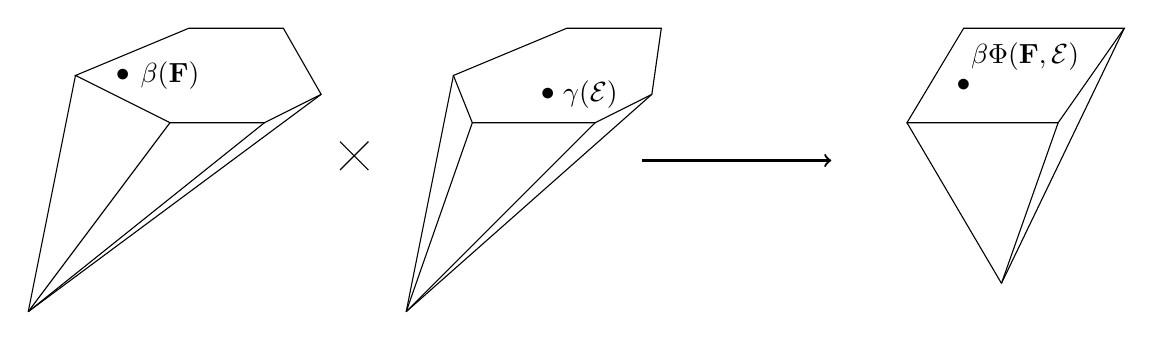
\begin{tikzpicture}[scale=1.2]
%% first cone
\draw[-](.5,.5)--(1,3);
\draw[-](.5,.5)--(2,2.5);
\draw[-](.5,.5)--(3,2.5);
\draw[-](.5,.5)--(3.6,2.8);
\draw(1.5,3.0) node {$\bullet$};
\draw(2.0,3.0) node {$\beta(\FF)$};
\draw[-](1,3)--(2,2.5)--(3,2.5)--(3.6,2.8)--(3.2,3.5)--(2.2,3.5)--cycle;
%% the cross
\draw[-] (3.8,2)--(4.1,2.3);
\draw[-] (4.1,2)--(3.8,2.3);
%% second cone
\draw[-](4.5,.5)--(5,3);
\draw[-](4.5,.5)--(5.2,2.5);
\draw(6.0,2.8) node {$\bullet$};
\draw(6.45,2.8) node {$\gamma(\cE)$};
\draw[-](4.5,.5)--(6.5,2.5);
\draw[-](4.5,.5)--(7.1,2.8);
\draw[-](5,3)--(5.2,2.5)--(6.5,2.5)--(7.1,2.8)--(7.2,3.5)--(6.2,3.5)--cycle;
%%the arrow
\draw[->,thick](7,2.1)--(9,2.1);
%% third cone
\draw[-](10.8,.8)--(9.8,2.5);
\draw[-](10.8,.8)--(11.4,2.5);
\draw[-](10.8,.8)--(12.1,3.5);
\draw(10.4,2.9) node {$\bullet$};
\draw(11.05,3.2) node {$\beta\Phi(\FF,\cE)$};
\draw[-](9.8,2.5)--(11.4,2.5)--(12.1,3.5)--(10.4,3.5)--cycle;
\end{tikzpicture}
\caption{The duality between Betti tables and cohomology tables involves three cones.  Namely, given the Betti table $\beta(\FF)$ of a complex of free $S$-modules, and the cohomology table $\gamma(\cE)$ of a complex of coherent sheaves on $\PP^n$, we use our pairing to produce the Betti table $\beta(\Phi(\FF,\cE))$ of a complex free $A$-modules. 
}
\label{fig:bracket}
\end{figure}





\addtocontents{toc}{\protect\setcounter{tocdepth}{-1}}
\subsection*{Comparing complexes and resolutions}
\addtocontents{toc}{\protect\setcounter{tocdepth}{1}}
% \subsecNTOC{Comparing Complexes and Resolutions}
Here is a consequence of the analysis of Betti tables allowed by this categorification. If every such complex were quasi-isomorphic to its homology---which is not the case except when $n=0$---then the Betti table of a complex would be the sum of the Betti tables of the resolutions of its homology.  We prove that similar decompositions happen much more generally, but they require rational coefficients,, not only integral ones, and the resolutions are generally not of the original homology modules. The denominators of the coefficients involved in the decomposition of $\beta(\FF)$ may be seen as a measure of the extent to which $\FF$ is not quasi-isomorphic to its homology. 

Theorem~\ref{thm:extremal rays refined} provides the full statement and proof, and implies the known results about decompositions of Betti tables
of resolutions from \cites{eis-schrey1,boij-sod2}.  Here is the special case of this result when the homology has finite length. By a (homologically) shifted resolution, we mean a complex of
finitely generated graded free modules the form
$$
\FF: F_{k}\leftarrow\cdots F_{k+\ell}\leftarrow 0
$$
that has homology only at $F_{k}$.
 
\begin{cor}\label{cor:decompose}
Let $\FF\in \DD^b(S)$ have finite length homology.  Then $\beta(\FF)$ is a positive rational combination of Betti tables of shifted free resolutions of modules of finite length. 
\end{cor}
As in the case of resolutions, the decomposition is algorithmic and, in a certain sense, unique.

We illustrate Corollary~\ref{cor:decompose} with an example.  By convention we display the Betti table of $\FF$ as a table
of integers where the element of the $i$-th column and $j$-th row is $\beta_{i,i+j}\FF$, and we replace each zero with $-$. For clarity we often decorate the $(0,0)$ entry
with a superscript $\circ$. In displays of complexes we often suppress the terms that are zero.

\begin{example}
Let $S=\kk[x,y]$ and consider the complex:
\[
\FF := \left[S^1\overset{\left(\begin{smallmatrix}x&y\end{smallmatrix}\right)}{\xlongleftarrow{\hspace*{1.1cm}}} S^2(-1)\overset{\left(\begin{smallmatrix}-y^2&xy\\xy&-x^2\end{smallmatrix}\right)}{\xlongleftarrow{\hspace*{1.1cm}}} S^2(-3)\overset{\left(\begin{smallmatrix}y\\x\end{smallmatrix}\right)}{\xlongleftarrow{\hspace*{1.1cm}}} S^1(-4)\right],
\]
which has has Betti table 
$$
\beta(\FF)=\begin{bmatrix} 1^\circ&2&-&-\\-&-&2&1\end{bmatrix}.
$$
The complex $\FF$ has finite length homology $H_{0}\FF = \kk,\ H_{1}\FF = \kk(-2)$. 

To decompose the Betti table of $\FF$, we consider the
modules $M:=S(-1)/(x^2,xy,y^2)$, and $N:=\Hom(M(1),\kk)$.  The Betti tables of (the minimal free resolutions of) $M[1]$ and $N$ are
\[
\beta(M[1])=\begin{bmatrix}
-^\zp&1&-&-\\
-&-&3&2
\end{bmatrix}
\quad \text{ and } \quad
\beta(N)=\begin{bmatrix}
2&3&-&-\\
-&-&1&-
\end{bmatrix},
\]
and we thus have the decomposition:
\[
\beta(\FF)=
\frac{1}{2}\beta(M[1])
+
\frac{1}{2}\beta(N).
\]


%To decompose the Betti table of $\FF$, we consider the
%complex 
%is
%\[
%\bG := 
%\left[S^1\overset{\left(\begin{smallmatrix}x^{2}&xy&y^{2}\end{smallmatrix}\right)}
%{\xlongleftarrow{\hspace*{1.1cm}}} 
%S^3(-2)\overset{\left(\begin{smallmatrix}y&0\\-x&y\\0&-x\end{smallmatrix}\right)}{\xlongleftarrow{\hspace*{1.1cm}}} S^2(-3)\right].
%\]
%The complex $\bG$ is the minimal free resolution of $S/(x,y)^{2}$, 
%Its dual $\bG^{*}$ is also a resolution, with Betti table
%$$
%\beta(\bG^{*}) = \begin{bmatrix} 2^\circ&3&-\\-&-&1\end{bmatrix}.
%$$
%\david{Really this is $\beta(\bG^{*}[-2]$. Do we care?}
%Thus
%\[
%\beta(\FF)=
%\frac{1}{2}\beta(\bG(1)[1])
%+
%\frac{1}{2}\beta(\bG^{*}).
%\]

We note that $\beta(\FF)$ can \emph{not} be written as a positive \emph{integral} combination of Betti tables of minimal resolutions of modules of finite length: First, $\beta(\FF)$ is not itself a resolution, since it has length 3 and $S$ has dimension only 2. 
Further,  the sum of the Betti numbers of any resolution of a nonzero $S$-module of finite length is at least 4, while the sum of the Betti numbers of $\FF$ is $6<2\cdot 4$.
\end{example}



%%%%%%%%%%%%%%%%%%%%%%%%%%%%%%
\subsection*{Beyond Polynomial Rings}
%%%%%%%%%%%%%%%%%%%%%%%%%%%%%%
%%%%%%%%%%%%%%%%%%%%%%%%%%%%%%
Our description of the cone of Betti tables of bounded complexes
extends to a wide class of rings in the following way. 
Let $S\subseteq R$ be a finite extension of graded rings, and let
$X=\Proj(R)$.  We let $f\colon X\to \PP^n$ denote the corresponding finite
map of projective schemes of dimension $n$, and we set $L:=f^*\cO(1)$.
%
%Write $R=R(X,L)=\oplus_{e\in \mathbb N} H^0(X,L^{\otimes e})$ for the \defi{section ring}
%of $L$.

%
%Our description of the cone of Betti tables of bounded complexes
%extends to a wide class of rings in the following way. 
%Let $f\colon X\to \PP^{n}$ be a finite morphism from a projective variety of dimension $n$, and set $L:=f^*\cO(1)$. 
%Write $R=R(X,L)=\oplus_{e\in \mathbb N} H^0(X,L^{\otimes e})$ for the \defi{section ring}
%of $L$.

We say that $\cU$ is an \defi{Ulrich sheaf} for $f$ if $f_*(\cU)\cong \cO_{\PP^n}^r$ for some $r>0$.  It was pointed out in \cite[Theorem~5]{eis-schrey-abel} that the existence of an Ulrich sheaf for $f$ implies that  the cone of cohomology tables of vector bundles on $X$ is the same as that on $\PP^{n}$. (The theorem is stated there when $L$ is very ample, but the proof
carries over to this more general situation.) 

The situation for Betti tables of resolutions over $R$ is not at all analogous to the situation of resolutions over $S$. But we prove a complete analogy for bounded complexes with finite length homology:

\begin{cor}\label{cor:isom cones}
Let $R$ be a graded $S$-algebra such that the map $f\colon \Proj(R)\to \P^{n}$ is finite.  If $\Proj(R)$ admits an Ulrich sheaf for $f$, then the cone of Betti tables
of bounded free complexes with finite length homology over  $R$ is the same
as the cone of complexes with finite length homology on $S$. 
\end{cor}

One direction of the proof is easy, as the pullback of an $S$-complex with finite length homology is an $R$-complex with finite length homology.  For the other direction we will use the duality statement of Theorem~\ref{thm:duality}.

\begin{example}\label{ex:elliptic}
Let $E$ be an elliptic curve and let $L=2P$, where $P$ is any point of $E$.  The map $f$ corresponding to the complete
linear series $|L|$ maps $E$ two-to-one to $\P^{1}$. The ring $R(E,L)$ has the form
$\kk[x_1,x_2,y]/(g(x_{1},x_{2},y))$  where $\deg(x_i)=1$, $\deg(y)=2$, and where $\deg(g)=4$.
If $P\neq Q\in E$ then the sheaf $L(P-Q)$ is an Ulrich sheaf for $f$. 

Thus the cone of
Betti tables of bounded free complexes with finite length homology over $R$ is the same
as the corresponding cone over $\kk[x_1,x_2]$.  A direct computation (see Example~\ref{ex:1441}) then implies that there is (up to scalar multiple), a minimal, exact complex of the form
\[
\cO_E\longleftarrow \begin{matrix}  \cO_E(-6P)^4\\ \oplus\\ \cO_E(-8P)^4\end{matrix}\longleftarrow \begin{matrix}  \cO_E(-8P)^4\\ \oplus\\ \cO_E(-10P)^4\end{matrix} \longleftarrow \cO_E(-16P)\longleftarrow 0.
\]
\end{example}

The bundle $L=f^*\cO_{\PP^n}(1)$ in Corollary~\ref{cor:isom cones} must be ample, since the map $L$ is finite.  However, the corollary does not hold for an arbitrary ample bundle.  For example, let $P$ be a point on an elliptic curve $E$, and let $R=R(E,P)$.  Since $\dim R_1=h^0(E,\cO_E(P))=1$, there cannot exist a pure complex:
\[
0\gets R^1\gets R^2(-1)\gets R(-2)\gets 0
\]
with finite length homology.

For all of the new graded rings $R$ covered by Corollary~\ref{cor:isom cones}, there exist finitely generated $R$-modules of infinite projective dimension.  It would thus be natural to consider bounded below elements of the derived category of graded $R$-modules.  In \S\ref{sec:infinite}, we take a different approach: by realizing an infinite resolution as a limit of bounded complexes, we apply our results to prove a decomposition theorem for the Betti table of certain infinite resolutions.

\subsection*{The Multigraded Case}
The functor $\Phi$ naturally generalizes to the multigraded case, offering the possibility of extending \BS theory to toric varieties.  Let $X$ be any projective toric variety with $\rank \Pic(X)=m$.  Let $R$ be the Cox Ring of $X$, presented as an $\mathbb N^m$-graded ring, and let $I$ be the irrelevant ideal of $R$.  Let $C=\kk[t_1, \dots, t_m]$ be $\mathbb N^m$-graded with irrelevant ideal $(t_1t_2\cdots t_m)$.  We say that a complex $\FF$ over $R$ or $C$ has \defi{irrelevant homology} if its homology is supported on the irrelevant ideal.

Let $\DD^b(R)$ and $\DD^b(C)$ denote the bounded derived categories of finitely generated, multigraded $R$-modules and $C$-modules, respectively.   For $\FF\in \DD^b(R)$ or in $\DD^b(C)$, $i\in \ZZ$, and $\alpha\in \ZZ^m$, we define the multigraded Betti numbers by the formula $\beta_{i,\alpha} \FF:=\dim \Tor_i(\FF,\kk)_{\alpha}$.  Similarly, for $\cE\in \DD^b(X), i\in \ZZ$ and $\alpha\in \ZZ^m$, we define multigraded cohomology numbers by the formula $\gamma_{i,\alpha} \cE:=\dim H^i(X, \cE(\alpha))$.  


For  $\FF\in \DD^b(R)$, let $\widetilde{\FF}$ denote the corresponding complex of coherent sheaves in $\DD^b(X)$.  We construct a functor
\[
\Phi_{X}: \DD^b(R)\times \DD^b(X)\to \DD^b(C)
\]
with the following properties:
\begin{theorem}\label{thm:Phimulti}
If $\FF$ is a multigraded complex of free graded $R$-modules and $\cE$ is a bounded complex of coherent sheaves on $X$, then:
\begin{enumerate} 
	\item\label{thm:Phi':1}  The multigraded Betti table of $\Phi_{X}(\FF,\cE)$ depends only on the multigraded Betti table of $\FF$ and the multigraded cohomology table of $\cE$.
	\item\label{thm:Phi':2}  If $\widetilde{\FF}\otimes \cE$ is exact, then $\Phi_{X}(\FF,\cE)$ has irrelevant homology.  
\end{enumerate}
\end{theorem}


Note that, if  $\FF$ is a complex with irrelevant homology and if $\cE$ is a vector bundle, then $\widetilde{\FF}\otimes \cE$ is always exact.
The functor $\Phi_{X}$ thus yields a pairing of the form:
\begin{equation*}%\tag{**}
\label{eqn:multipairing}
%
\left\{\begin{matrix}
%\text{Cone generated by}\\
\text{Multigraded Betti tables} \\ \text{of free $R$-complexes}\\
\text{with irrelevant homology}\end{matrix}\right\}
%
\times 
%
\left\{\begin{matrix}
%\text{Cone generated by}\\
\text{cohomology }\\
\text{tables of vector}\\
\text{ bundles on } X
\end{matrix}\right\}
%
\longrightarrow
\left\{\begin{matrix}
%\text{Cone generated by}\\
\text{Multigraded Betti tables} \\ \text{with  free $C$-complexes}\\
\text{with irrelevant homology}
\end{matrix}\right\}
\end{equation*}
As we discuss in \S\ref{sec:toric}, the target of this pairing, that is, the cone of free $C$-complexes with irrelevant homology, is simpler than the cone of free resolutions of over $C$.  This enables the construction of toric/multigraded analogues of the Eisenbud--Schreyer functionals, and it thus seems that the cone of free $R$-complexes with irrelevant homology will be easier to study than the cone of free resolutions over $R$. 

%%%%%%%%%%%%%%%%%%%%%%%%
%%%%%%%%%%%%%%%%%%%%%%%%
\addtocontents{toc}{\protect\setcounter{tocdepth}{-1}}
\section*{Acknowledgments}
\addtocontents{toc}{\protect\setcounter{tocdepth}{1}}
%%%%%%%%%%%%%%%%%%%%%%%%
%%%%%%%%%%%%%%%%%%%%%%%%
We thank Christine Berkesch, Bhargav Bhatt, Rob Lazarsfeld, Ezra Miller, and Ravi Vakil for conversations and suggestions that improved this paper.
Some of this work was completed during the first author's visit to the University of Michigan, and we are grateful for their hospitality.  The computer
algebra system \texttt{Macaulay2} \cite{M2} provided valuable assistance throughout our work.
%Courtney Gibbons?  Jesse Burke?

%%%%%%%%%%%%%%%%%%%%%%%%
%%%%%%%%%%%%%%%%%%%%%%%%
\section*{\underline{{Part I: Categorifying the Duality in \BS Theory}}}
%%%%%%%%%%%%%%%%%%%%%%%%
%%%%%%%%%%%%%%%%%%%%%%%%
\section{Background and notation}\label{sec:notation}
%%%%%%%%%%%%%%%%%%%%%%%%
%%%%%%%%%%%%%%%%%%%%%%%%
We gather some notation and definitions that we will use throughout.  We set $\mathfrak m=(x_0, \dots, x_n)$ to be the homogeneous maximal ideal on $S$.
\begin{defn}
If $\FF\in \DD^b(S)$ is a free complex, then we say that $\FF$ is \defi{minimal} if each differential $\partial: \FF_i\to \FF_{i-1}$ satisfies $\partial(\FF_i)\subseteq \mathfrak m\FF_{i-1}$.
\end{defn}
We may represent any $\FF\in \DD^b(S)$ by a minimal, free complex.  Under this assumption, we may write $\FF_i$ as the direct sum $\FF_i=\oplus_{j\in \ZZ} S(-j)^{\beta_{i,j}\FF}$.  If $\FF$ is quasi-isomorphic to a complex with only one nonzero term, then we say that $\FF$ is a \defi{shifted resolution}.  We use the notation $\HH_r\FF$ to denote the $r$th homology module of $\FF$.

\begin{defn}\label{def:deg seq}
A \defi{ degree sequence of codimension $\ell$} is a sequence
\[{\dd}=(\dots, d_i, d_{i+1}, \dots)
\]
with  $d_{i} \in \{-\infty\}\cup \ZZ\cup \{\infty\}$ and $d_i \leq d_{i+1}-1$ and 
where there are precisely $\ell+1$ entries of $\dd$ lying in $\ZZ$. 
We define a partial order on shifted degree sequences by the termwise partial order, so $d\leq d'$ if $d_i\leq d_i'$ for all $i$.
\end{defn}
Note that this usage is slightly more general than that of \cite{eis-schrey1} or \cite{boij-sod2}, where degree
sequences were taken to be what would be written here as
$(\dots,-infty,d_{0}^{\zp,\dots,d_{\ell}, \infty,\dots}$.

As with Betti tables, we use a $\zp$ to indicate homological position zero when writing a degree sequence. 
Thus for example
$$
(\dots, -\infty , 0, 1^{\circ}, 3, \infty, \dots) < (\dots, -\infty , 0, 1, 3^{\circ}, \infty, \dots) 
$$
are  degree sequences of codimension 2.

Given any degree sequence $\dd$, we say that a complex $\FF$ is \defi{pure of type $\dd$} if, for all $i$ such that $d_i\in \ZZ$, the free module $\FF_i$ is generated entirely in degree $d_i$.   The existence of pure resolutions (see~\cite{efw} or \cite[\S5]{eis-schrey1}) shows that, for any  degree sequence $\dd$ of codimension $\ell\leq n+1$, there exists a shifted resolution of a Cohen-Macaulay module over $S$ that is a pure complex of type $\dd$.  One of the central results of \BS theory is that the Betti tables of pure resolutions correspond bijectively with the extremal rays of cone of Betti tables of minimal free resolutions.  In other words, if $\FF$ is a minimal free resolution, then $\beta(\FF)$ may be written as a positive rational combination of the Betti tables of pure resolutions.  See~\cites{eis-schrey-icm,floystad-expository} for expository introductions to \BS theory.  We remark that, in \S\ref{sec:refined}, we introduce new notation for discussing many different cones of Betti tables.


If $P$ is some property that may be applied to a graded $S$-module, we extend the definition to the derived category by saying that $\FF \in \DD^b(S)$ has property $P$ if the direct sum of the homology modules of $\FF$ have this property. We similarly extend the definition of any property of coherent sheaves to elements $\cE\in \DD^b(\PP^n)$.  

A \defi{root sequence $f$ of dimension $s$} is a strictly decreasing sequence
of $s$ integers, $f=(f_1>\cdots>f_s)$.  
A sheaf $\cE$ on $\PP^{n}$ is
\defi{supernatural of type} $f=(f_1, \dots, f_{s})$ if the following are satisfied: 
\begin{enumerate}
\item The dimension of $\cE$ is $s$.
\item For all $j\in \mathbb Z$, there exists at most one $i$ 
		such that $\dim_\Bbbk H^i(\PP^{n}, \cE(j))\ne 0$.
\item The Hilbert polynomial of $\cE$ has roots $f_1, \dots, f_{s}$.
\end{enumerate}
For every root sequence $f$, there exists a supernatural sheaf of type
$f$~\cite[Theorem~0.4]{eis-schrey1}.
Moreover, the cohomology table of any coherent sheaf 
can be written as a positive real combination of cohomology tables 
of supernatural sheaves~\cite[Theorem~0.1]{eis-schrey1}.  

One of the main results of \cite{eis-schrey1} indicates a duality between the cone of Betti tables of free resolutions of finite length graded $S$-modules and the cone of cohomology tables of vector bundles on $\PP^n$.  We provide a new perspective on this duality in \S\ref{sec:duality}. 


\begin{defn}
We index complexes in $\DD^b(S)$ homologically as in $\FF=[\dots \gets \FF_0\gets \FF_1\gets \dots]$.  For any $k\in \ZZ$, we define a \defi{shift} of $\FF$, denoted $\FF[k]$, as the complex obtained by shifting the indices in the following way:  $(\FF[k])_i=\FF_{i-k}$.
\end{defn}


%%%%%%%%%%%%%%%%%%%%%%%%
%%%%%%%%%%%%%%%%%%%%%%%%
\section{A duality pairing for \BS Theory}\label{sec:duality pairing}
%%%%%%%%%%%%%%%%%%%%%%%%
%%%%%%%%%%%%%%%%%%%%%%%%
In this section we define the functor $\Phi$ and we prove Theorem~\ref{thm:Phi} describing its main properties.  As before, set $A= \kk[t]$. Let 
$\sigma\colon S\to S\otimes A = S[t]$
be the homomorphism defined by $\sigma(x_{i})=x_{i}t$. 
We write $-\otimes_\sigma S[t]$ to denote tensoring over $S$ with $S[t]$ using the structure
given by $\sigma$. Note that $\sigma$ is not a flat map---it is not even equidimensional.

If $F$ is a graded  $S$-module, then 
$$
F\otimes_{\sigma} S[t]
$$
is a bigraded $S[t]$ module.
Thus we may define a functor $\tau$ on derived
categories that takes a graded complex of free $S$-modules $\FF$ to
$$
\tau(\FF): =\widetilde \FF \otimes_{\sigma}\cO_{\PP^{n}\times \AA^{1}},
$$
a complex of graded sheaves on $\PP^{n}\times \AA^{1}$, with the grading coming from degree in $t$, the coordinate on $\AA^{1}$. For example, if 
$$
\FF= [\xymatrix{0&S\ar[l]&S(-e)\ar[l]_f& 0\ar[l]}]
$$
where $f$ is a form of degree $e$, then
$$
\tau(\FF)= [\xymatrix{0&\cO_{\PP^{n}}\boxtimes A\ar[l]&\cO_{\PP^{n}}(-e)\boxtimes A(-e)\ar[l]_-{t^ef}& 0\ar[l]}]
$$
where $P\boxtimes Q$ denotes the tensor product of the pullbacks of $P$ and $Q$ from
$\PP^{n}$ and $\AA^{1}$, respectively. This description of $\tau$ could 
be extended to graded complexes of arbitrary finitely generated graded modules
at the expense of replacing the tensor product with a derived tensor product, but we
will never need this.

%\begin{defn} The functor $\Phi: D^{b}(\P^{n}) \times D^{b}(S) \to D^{b}(A)$ is given by:
%$$
%\Phi(\cE,\FF) = R\pi_{*} \left(\tau_{0}(\cE)\otimes_{\P^{n}\times\AA^{1}} \tau_{1}(\FF)\right)
%$$
%where $\pi: \PP^{n}\times \AA^{1}\to \AA^{1}$ is the projection.
%\end{defn}

\begin{defn} \label{defn:product} The functor $\Phi: \DD^{b}(S)\times \DD^b(\PP^n) \to \DD^{b}(A)$ is given by:
$$
\Phi(\FF,\cE) = Rp_{2*} \bigl(\tau(\FF)\otimes_{\P^{n}\times\AA^{1}} (\cE\boxtimes \cO_{\AA^{1}}) \bigr)
$$
where $\FF$ denotes a graded  complex of finitely generated free $S$-modules and
$p_2: \PP^{n}\times \AA^{1}\to \AA^{1}$ is the projection. We  often write
$\FF\cdot \cE$ for $\Phi(\FF,\cE)$.
\end{defn}

For those comfortable with stacks, Definition~\ref{defn:product}
could be rephrased as follows. Consider the commutative diagram:
\[
\xymatrix{
\PP^n&\PP^{n}\times [\AA^1/\GG_m]\ar[l]_-{\pi_{1}} \ar[r]^-{\Sigma} \ar[d]^{\pi_2}&[\AA^{n+1}/\GG_m]\\
&[\AA^1/\GG_m]&%[\Spec(\kk)/\GG_m]\ar[l]_{o}
}
\]
where $\Sigma$ is the morphism induced by $\sigma$ and the maps $\pi_1$ and $\pi_2$ are the projections.  We could define $\Phi(\FF,\cE)$ to be $R\pi_{2*}\left( \Sigma^*\FF\otimes \pi_{1}^{*}\cE\right)\in \DD^b([\AA^1/\GG_m])$.

To see why this is an equivalent definition, note first  that there is an equivalence of categories (given by pullback/descent) between coherent sheaves on $[\AA^1/\GG_m]$ and graded, finitely generated $A$-modules. Further, since the covering map $\AA^1\to [\AA^1/\GG_m]$ is flat, cohomology commutes with base change (see \cite[0765]{stacks-project}) for the diagram
\[
\xymatrix{
\PP^n\times \AA^1\ar[r]\ar[d]^-{p_2}&\PP^{n}\times [\AA^1/\GG_m]\ar[d]^{\pi_2}\\
\AA^1\ar[r]&[\AA^1/\GG_m].
}
\]
Thus, the pullback of $R\pi_{2*}\left( \Sigma^*\FF\otimes \pi_{1}^{*}\cE\right)$ is quasi-isomorphic 
to $\Phi(\FF,\cE)$ as defined in Definition \ref{defn:product}.

Here is a sample computation of $\Phi$: 

\begin{example} Let 
$$
\bK = \bigl[ S\lTo S^{n+1}(-1) \lTo \wedge^{2}(S^{n+1})(-2) \lTo\cdots\lTo S(-n-1)\bigr]
$$
be the Koszul complex, the minimal free resolution of $\kk$, and take
$\cE = \cO_{\PP^{n}}$, so that 
$$
\bK \cdot \cE = Rp_{2*}\tau(\bK).$$  
There is a spectral sequence
\[
E_2^{i,-j}=H^i(\widetilde{\bK_j})\otimes A(-j))\Rightarrow R^{i-j}p_{2*}(\tau(\bK)).
\]
But 
%since $E_1^{i,-j}\ne 0$ only
%$$
%\widetilde {\sigma^{*} S(-a)} \cong \cO_{\PP^{n}}(-a)\otimes A(-a),
%$$
the terms on this page all vanish except for
$$
E^{0,0}_2= H^{0}(\cO_{\PP^{n}})\otimes A = A,
$$
in homological degree 0, and 
$$
E^{n+1,-n}=H^{n}(\cO_{\PP^{n}}(-n-1)) \otimes  A(-n-1) = A(-n-1)
$$
in homological degree $(n+1)-n = -1$.
Thus the complex $\bK \cdot \cE$ has the form
$$
A\lTo^{ut^{n}}A(-n-1)
$$
for some $u\in \kk$. But the complex $\FF$ has homology of finite length, so the complex $\sigma^{*}\FF \otimes p_{2}^{*}\cE$ has homology annihilated by a power of $t$, and thus $\FF\cdot \cE$ will also have homology annihilated by a power of $t$. It follows that $u\neq 0$, and $\FF\cdot \cO_{\PP^{n}}$ is quasi-isomorphic to the graded $A$-module $A/(t^{n})$, regarded as a complex concentrated in homological degree 0.
\end{example}


%%%%%%%%%%%%%%%%%%%%%%%%%
%%%%%%%%%%%%%%%%%%%%%%%%%
%\section{The Betti table of $\Phi(\FF,\cE)$}\label{sec:Betti of Phi}
%%%%%%%%%%%%%%%%%%%%%%%%%
%%%%%%%%%%%%%%%%%%%%%%%%%
The following result is a strengthened version of Theorem~\ref{thm:Phi}\eqref{thm:Phi:1}.
\begin{theorem}\label{thm:betti numbers of pairing}
The Betti numbers of $\FF\cdot \cE = \Phi(\FF,\cE)$ are given by the formula:
\[
\beta_{i,j}(\FF\cdot \cE)=\sum_{\substack{p-q=i\\ j\in \ZZ}}  \beta_{p,j}(\FF)\gamma_{q,-j}(\cE).
\]
In particular, the Betti table of $\FF\cdot \cE$ only depends on $\beta(\FF)$ and $\gamma(\cE)$.
\end{theorem}


\begin{proof}
Without loss of generality, we assume that $\FF$ is a minimal free complex supported entirely in nonnegative homological degrees, so that $\FF=[\FF_0\gets \dots \gets \FF_p]$.  
We may compute $\FF\cdot \cE$ explicitly in terms of a certain spectral sequence for computing $Rp_{2*}$.  First, we consider the double complex $C_{\bullet, \bullet}$ where $C_{i,\bullet}$ is the Cech resolution of $\left( \tau(\FF_i)\otimes_{\PP^n_A} (\cE\boxtimes \cO_{\AA^1})\right)$ on $\PP^n_A$ with respect to the standard Cech cover of $\mathbb P^n$.  If we represent all of the maps in $C_{\bullet, \bullet}$ with matrices, then all of the vertical maps (which are induced by the Cech resolutions) will involve bidegree $(0,0)$ elements, and all of the horizontal maps (which are induced by the maps in $\tau(\FF)$) will involve bihomogeneous elements that are strictly positive in both bidegrees.

Since $\Tot(C_{\bullet, \bullet})$ is a complex of flat $A$-modules that is quasi-isomorphic to $\FF\cdot \cE$, we can obtain the Betti numbers by computing $\Tor(\Tot(C_{\bullet, \bullet}), A/(t))$.  When we tensor by $A/(t)$, the vertical maps of $C_{\bullet, \bullet}$ are unchanged, but the horizontal maps all go to $0$.  
Hence, one spectral sequence degenerates, so the $i$th homology of $\Tot(C_{\bullet,\bullet})/(t)$ equals the sum 
\[
\HH^i(\Tot(C_{\bullet,\bullet})/(t))\cong \bigoplus_{j} \HH^j_{\text{vert}}(C_{i+j,\bullet})
\]

Now we compute the other spectral sequence.
Recall that $\FF_i=\oplus_{j\in \ZZ} S(-j)^{\beta_{i,j}(\FF)}$.  For brevity, we use $\beta_{i,j}:=\beta_{i,j}(\FF)$, and we may write $\FF_i'\otimes \cE\cong \bigoplus_{j\in \ZZ} \cE(-j)^{\beta_{i,j}}\boxtimes A(-j)^{\beta_{i,j}}$.

After taking the vertical homology of $C_{\bullet, \bullet}$, we obtain:
\[
\xymatrix{
\bigoplus_{j} H^n(\cE(-j)^{\beta_{0,j}})\otimes A(-j)^{\beta_{0,j}}&\bigoplus_{j} H^n(\cE(-j)^{\beta_{1,j}})\otimes A(-j)^{\beta_{1,j}}\ar[l]&\dots\ar[l]\\
\vdots & \vdots&\\
\bigoplus_{j} H^1(\cE(-j)^{\beta_{0,j}})\otimes A(-j)^{\beta_{0,j}}&\bigoplus_{j} H^1(\cE(-j)^{\beta_{1,j}})\otimes A(-j)^{\beta_{1,j}}\ar[l]&\dots\ar[l]\\
\bigoplus_{j} H^0( \cE(-j)^{\beta_{0,j}})\otimes A(-j)^{\beta_{0,j}}&\bigoplus_{j} H^0(\cE(-j)^{\beta_{1,j}})\otimes A(-j)^{\beta_{1,j}}\ar[l]&\dots\ar[l]
}
\]
We conclude that
\[
\Tor^i_A(\FF\cdot \cE, A/(t))\cong \HH^i(\Tot(C_{\bullet,\bullet})/(t))\cong \bigoplus_{p-q=i} \bigoplus_{j} H^q(\cO(-j)^{\beta_{p,j}}\otimes \cE)\otimes A(-j)^{\beta_{p,j}},
\]
which proves the formula.
\end{proof}


\begin{example}\label{ex:1441}
Let $S=\kk[x,y,z]$ and let
\begin{equation}\label{eqn:intro ex}
\beta(\FF)=\begin{bmatrix} 1&-&-&-\\ -&-&-&-\\-&4&4&-\\-&4&4&-\\-&-&-&-\\-&-&-&1 \end{bmatrix}.
\end{equation}

No multiple of the Betti table $\beta(\FF)$ cannot equal the Betti table of a minimal, free complex with finite length homology. Indeed, such a complex would be a resolution,  so this case is covered by the theory of \cite{Eis-Schr}. But it is instructive to see how this follows directly from
Theorem~\ref{thm:Phi}:

If $\cE$ to be a rank $8$ supernatural bundle of type $(0,-8)$ then 
$\FF\cdot \cE$ would be a minimal complex of the form
\[
\FF\cdot \cE=\left[ \begin{matrix}A(-3)^{240}\\ \oplus \\A(-4)^{256}\end{matrix} \longleftarrow \begin{matrix}A(-4)^{256}\\\oplus \\ A(-5)^{240}\end{matrix}\right].
\]
Since the complex is minimal, the kernel of the map will contain a subsheaf of $A(-4)^{256}$ of rank at least $256-240=16$, and hence $\FF\cdot \cE$ cannot have finite length homology, and  by Theorem~\ref{thm:Phi}\eqref{thm:Phi:2} it follows that no multiple of $\beta(\FF)$ can be the Betti table of a complex with finite length homology. However, we shall see in Example~\ref{ex:1441bis} that 
there that $10\beta(\FF)$ is the Betti table of a complex with 1-dimensional homology.
\end{example}

As a Corollary of Theorem~\ref{thm:betti numbers of pairing}, we can use $\Phi$ to recover the Betti numbers of $\FF$  or the cohomology
table of $\cE$:
\begin{cor} Let $\FF\in \DD^b(S)$ and let $\cE\in \DD^b(\PP^n)$.
\begin{enumerate}
\item 
 $\beta_{i,j}(\FF) = \beta_{i,j}(\FF\cdot \cO_{\P^{n}}(j))$ for all $i,j$, where $\cO_{\PP^n}(j)$ is regarded as a complex concentrated in homological degree 0.
\item $h^{i}(\cE(j)) = \beta_{-i,-j}(S(j)\cdot \cE)$, for all $i,j$, where $S(j)$ is regarded as a complex concentrated in homological degree 0.
\end{enumerate}
%\qed
\end{cor}



We will focus in this paper on free complexes, and we will need to use the definition of $\Phi$
only in the special case where $\cE$ is (the extension by zero of) a vector bundle on a linear subspace of $\PP^n$.
\begin{prop}\label{prop:exact}
Let $\FF\in \DD^b(S)$ and $\cE\in \DD^b(\PP^n)$.  If $\widetilde \FF\otimes \cE$ is exact, then the homology of the complex $\Phi(\FF,\cE)$ has finite length.
\end{prop}

\begin{proof} It suffices to show that the homology of $\Phi(\FF,\cE)$ is annihilated by
a power of $t$. After inverting $t$ the map $\sigma$ becomes the usual inclusion $S\subset S[t,t^{-1}]$
composed with the invertible change of variables $x_{i}\mapsto x_{i}t$. Thus the complex 
$$
\Gbull:=\bigl(\widetilde\FF\otimes_{\sigma}\cO_{\PP^{n}\times \Spec A[t,t^{-1}]}\bigr)
\otimes_{\PP^{n}\times \Spec A[t,t^{-1}]}
\cE \cong \widetilde \FF \otimes \cE \otimes \cO_{\Spec A[t,t^{-1}]}
$$
has no homology. It follows by a spectral sequence computation that 
the complex $R\pi_{2*}\GG$ on $\Spec A[t,t^{-1}]$ has no homology. By flat base change,
this is equal to the restriction of $\Phi(\FF,\cE)$ on the open set $t^{-1}$, and we see that the homology
of $\Phi(\FF,\cE)$ is annihilated by a power of $t$, as required.
\end{proof}
%
%\begin{example}\label{ex:sup1}
%On $\PP^2$, let $\cE$ be a supernatural bundle of type $(1,-3)$ and rank $2$.  The map $\beta(\FF)\mapsto \beta(\FF\cdot \cE)$ takes a Betti table on $S$ and produces a Betti table on $A$, and we may describe this map as follows.  Fix some $i,j\in \ZZ$ and let $\FF$ be the one-term complex $\FF=S^\alpha(-j)[i]$.  Since $\cE$ is supernatural, for any $j\in \ZZ\setminus \{3,-1\}$, there is a unique $\ell_j\in \{0,1,2\}$ such that $h^{\ell_j}(\cE(-j))\ne 0$.   Then $\FF\cdot \cE$ is the one-term complex with $\beta_{i-\ell_j,j}(\FF\cdot \cE)=\gamma_{\ell_j,j}\cdot \alpha.$
%
%We represent this map as matrix by writing $\left( \gamma_{\ell_j,j}\cE\right)[-\ell_j]$
%\david{should this be $\gamma_{\ell_j,j}(\cE[-\ell_j])$?? Clarify the notation.}
% in position $(i,j)$.  For instance, with $\cE$ as above, we have
%\[
%%\beta(-\cdot \cE)\Rightarrow
%\begin{pmatrix}
%&\vdots&\vdots&&\vdots&\\
%\dots&\gamma_{0,3}&\gamma_{0,2}&0&\dots\\
%\dots&\gamma_{0,2}&0&\gamma_{1,0}[-1]&\dots\\
%\dots&0&\gamma_{1,0}[-1]&\gamma_{1,-1}[-1]&\dots\\
%\dots&\gamma_{1,0}^\zp[-1]&\gamma_{1,-1}[-1]&\gamma_{1,-2}[-1]&\dots\\
%\dots&\gamma_{1,-1}[-1]&\gamma_{1,-2}[-1]&0&\dots\\
%\dots&\gamma_{1,-2}[-1]&0&\gamma_{2,-4}[-2]&\dots\\
%%\dots&0&5[-2]&12[-2]&\dots\\
%&\vdots&\vdots&&\vdots&\\
%\end{pmatrix}
%=
%\begin{pmatrix}
%&\vdots&\vdots&&\vdots&\\
%\dots&12&5&0&\dots\\
%\dots&5&0&3[-1]&\dots\\
%\dots&0&3[-1]&4[-1]&\dots\\
%\dots&3^\zp[-1]&4[-1]&3[-1]&\dots\\
%\dots&4[-1]&3[-1]&0&\dots\\
%\dots&3[-1]&0&5[-2]&\dots\\
%%\dots&0&5[-2]&12[-2]&\dots\\
%&\vdots&\vdots&&\vdots&\\
%\end{pmatrix}.
%\]
%\end{example}


%%%%%%%%%%%%%%%%%%%%%%%%%%%%%%%%%%%%%%%%%
%%%%%%%%%%%%%%%%%%%%%%%%%%%%%%%%%%%%%%%%%
\section{Categorified Eisenbud--Schreyer functionals}\label{sec:functionals}
%%%%%%%%%%%%%%%%%%%%%%%%%%%%%%%%%%%%%%%%%
%%%%%%%%%%%%%%%%%%%%%%%%%%%%%%%%%%%%%%%%%
We now illustrate how the pairing $\Phi$ provides a unifying view on the Eisenbud--Schreyer functionals and  the corresponding positivity results, such as~\cite[Positivity 1 and 2]{eis-schrey-icm}.  The basic idea can be envisioned via Figure~\ref{fig:bracket} or equation \eqref{eqn:**}.  First, we use $\Phi$ to obtain a  bilinear pairing that takes a Betti table $\beta(\FF)$ and a cohomology table $\gamma(\cE)$ to a Betti table $\beta(\FF\cdot \cE)$ on $A$.  Second, we analyze the functionals on $\DD^b(A)$ which are nonnegative when evaluated on complexes with finite length homology.  
This recipe provides lots of functionals that are nonnegative on Betti tables, including all of the Eisenbud--Schreyer functionals $\langle -, -\rangle_{\tau,\kappa}$ (see ~\cite{eis-schrey-icm} for the definition, and for results about these functionals.)


\begin{remark}
We refer throughout to the definition of $\langle -, -\rangle_{\tau,\kappa}$ given in \cite{eis-schrey-icm}, which is slightly different than the definition from \cite{eis-schrey1}.
\end{remark}

\begin{defn}\label{defn:chi}
Given $\Gbull\in \DD^b(A)$, we define $\chi_{i,j}(\Gbull)=\chi_{i,j}(\beta(\Gbull))$ to be the dot product of the Betti table $\beta(\Gbull)$ with
\begin{equation}\label{eqn:chi}
\chi_{i,j}:=
\left|
\begin{array}{cccccccc}
 & \vdots& &\multicolumn{1}{|c}{\vdots}&& \vdots&&\\
\dots&0&0&\multicolumn{1}{|c}{1}&-1&1&-1&\dots\\
\dots&0&0&\multicolumn{1}{|c}{1}&-1&1&-1&\dots\\
\dots&0&0&\multicolumn{1}{|c}{\mathbf{1}}&-1&1&-1&\dots\\ \cline{4-5}
\dots&0&0&0&0&\multicolumn{1}{|c}{1}&-1&\dots\\
\dots&0&0&0&0&\multicolumn{1}{|c}{1}&-1&\dots\\
& \vdots&&\vdots&& \multicolumn{1}{|c}{\vdots}&&\\
\end{array}
\right|
\end{equation}
where the boldface $1$ corresponds to $\beta_{i,j}$; that is, the boldface $1$ is in column $i$ and row $i-j$. 
\end{defn}
The line that snakes through
the table indicates how $\chi_{i,j}$ separates a Betti into two regions.  In the upper region, this is simply computing an Euler characteristic, and in the lower region, it is dot product with the zero matrix. The functionals $\langle - , \cE \rangle_{\tau,\kappa}$ used previously in Boij-S\"oderberg theory, where $\cE$ is a supernatural sheaf, can be expressed in terms of the $\chi_{i,j}$. 
This is the sense in which the complex of $A$-modules $\Phi(\FF,\cE)$ categorifies the Eisenbud--Schreyer functionals.

\david{the indexing in the following is significantly off from that of \cite{eis-schrey1}: There the
functionals are called $\langle -,-\rangle_{c,\tau}$ and $c\in \ZZ$ while $\tau \in [0,n]$---backwards
from what's below. I think it's enough to reverse the $\tau$ and $\kappa$ below, but we
ought to rename $\kappa$ as $c$ for consistency. I have NOT yet made this change.}
\begin{prop}\label{thm:categorified:2}
Let $\cE$ be a supernatural sheaf of dimension $s$ on $\PP^n$ with root sequence $f$, and let $\FF$ be a bounded minimal free complex. Fix any $1\leq \tau\leq s$ and $\kappa\in \ZZ$.  There exists $\nu\in \ZZ$ such that
\[
\langle \FF, \cE\rangle_{\tau,\kappa}= 
 \chi_{0, \nu}(\FF\cdot \cE).
\]
\end{prop}

\begin{proof} 
We set $\nu:=\min\{\max\{\kappa, -f_{\tau}-1\},-f_{\tau+1}-1\}$.  It suffices to verify the claim for one-term complexes of the form $\FF=S^1(-u)[v]$, with $u$ and $v$ arbitrary.  
If we set $f_0=\infty$ and $f_{s+1}=-\infty$, then there exists a unique $p$ such that $f_p\geq -u>f_{p+1}$, and thus  $\beta_{v-p,u}(\FF\cdot \cE)=\gamma_{p,-u}(\cE)$ while all other Betti numbers  of $\FF\cdot \cE$ are equal to $0$.  (If $-u$ is a root of $f$, then both functionals are trivially zero, and we henceforth assuem that $-u$ is not a root of $f$.)


Hence $\chi_{0, \nu}(\FF\cdot \cE)$ is either $(-1)^{v-p}\gamma_{p,-u}(\cE)$ or $0$, depending on whether or not the $1$-term complex of $\FF\cdot \cE$ lies in the ``upper'' or ``lower'' region of $\chi_{0,\nu}$.  Similarly, one may check from the definition in \cite{eis-schrey-icm} that $\langle \beta(\FF),\gamma(\cE)\rangle_{\tau,\kappa}$ is either $(-1)^{v-p}\gamma_{p,-u}(\cE)$ or $0$.  
It thus suffices to confirm that our two functionals are nonzero in precisely the same situations.  We first consider the case when $v-p<0$.  Then $\FF\cdot \cE$ is supported in homological degrees $<0$, and hence $\chi_{0, \min\{\kappa,\; -f_{\tau}-1\}}(\FF\cdot \cE)$ is automatically $0$. Similarly, since $v<p$ there no terms in the definition of $\langle \beta(\FF),\gamma(\cE)\rangle_{\tau,\kappa}$ of the form $\beta_{v,u}\gamma_{p,-u}$, and hence this functional is also zero.  

It is similarly routine to check that, if $v-p>1$, then both functionals are nonzero.  We are then left with the cases $v-p=0$ and $v-p=1$.  For $v-p=0$, we have:
\begin{equation}\label{eqn:cond1}
\langle \beta(\FF),\gamma(\cE)\rangle_{\tau,\kappa}=0 \iff p> \tau \text{ or } p=\tau \text{ and } u>\kappa.
\end{equation}
We also have
\begin{equation}\label{eqn:cond2}
\chi_{0,\nu}(\FF\cdot \cE)=0 \iff u> \nu=\min\{\max\{\kappa, -f_{\tau}-1\},-f_{\tau+1}-1\}.
\end{equation}
We observe that the conditions in \eqref{eqn:cond1} and \eqref{eqn:cond2} are equivalent.  Namely, the second condition yields that either: $f_{\tau+1}\geq-u$ (which is equivalent to $p>\tau$); or $u>\kappa$ and $f_{\tau}\geq -u$ (which is equivalent to $p\geq \tau$ and $u>\kappa$). 

We now check the case $v-p=1$.  Here we have:
\begin{equation}\label{eqn:cond3}
\langle \beta(\FF),\gamma(\cE)\rangle_{\tau,\kappa}=0 \iff p> \tau \text{ or } p=\tau \text{ and } u>\kappa+1.
\end{equation}
We also have
\begin{equation}\label{eqn:cond4}
\chi_{0,\nu}(\FF\cdot \cE)=0 \iff u> \nu+1=\min\{\max\{\kappa+1, -f_{\tau}\},-f_{\tau+1}\}.
\end{equation}
Again, these conditions are equivalent: $f_{\tau+1}>-u$ (which, given that $-u$ is not a root of $\cE$, is equivalent to $p>\tau$); or $u>\kappa+1$ and $f_{\tau}>-u$ (which, given that $-u$ is not a root of $\cE$, is equivalent to $p\geq \tau$ and $u>\kappa$). 
\end{proof}

We define $\DD^b(A)_{\text{tor}}$ as the subcategory of $\DD^b(A)$ consisting of complexes whose homology is torsion.
The usefulness of the functionals $\chi_{i,j}$ comes from a positivity result generalizing that of \cite{eis-schrey1}:

\begin{thm}\label{thm:categorified}\label{thm:categorified:1}  Let $\FF\in \DD^b(S)$ and $\cE\in \DD^b(\PP^n)$. If  $\codim(\FF)+\codim(\cE)\geq n+1$, then
\[
\chi_{i,j}(\FF\cdot \cE)\geq 0
\]
\end{thm}

%\begin{thm}\label{thm:categorified}\david{the two parts really don't belong together; make into two results}
%\begin{enumerate}
%	\item\label{thm:categorified:1}  Let $\FF\in \DD^b(S)$ and $\cE\in \DD^b(\PP^n)$ with $\codim(\FF)+\codim(\cE)\geq n+1$.  Then
%\[
%\chi_{i,j}(\FF\cdot \cE)\geq 0
%\]
%	\item\label{thm:categorified:2}  \david{this needs fixing: a sheaf of codim $s$ would have
%	root sequence with $n-s$ terms.} Let $\cE$ be a supernatural sheaf of codimension $s$ on $\PP^n$ with root sequence $f$.  Fix $1\leq \tau \leq s$ and $\kappa\in \ZZ$.  If we set $\nu:=\min\{\kappa, f_{\tau}-1\}$,
%	%there exists $\nu \in \ZZ$ such that 
%	then we have an equality of functions:
%\[
%\bigg( \beta(\FF)\mapsto \chi_{0,\nu}(\FF\cdot \cE_f)\bigg) =\bigg( \beta(\FF)\mapsto \langle \FF, \cE_f\rangle_{\tau,\kappa} \bigg).
%\]
%%from $\VV \to \QQ$, where $\langle -, \cE_{f}\rangle_{\tau,\kappa}$ is the functional defined in \cite{eis-schrey-icm}, extended in the natural way to all of $\VV$.
%\end{enumerate}
%\end{thm}


\begin{proof}
The number $\chi_{i,j}(\FF\cdot \cE)$ only depends on the Betti table of $\FF\cdot \cE$, which by Theorem~\ref{thm:Phi}\eqref{thm:Phi:1} only depends on $\beta(\FF)$ and $\gamma(\cE)$.  We may thus assume that $\kk$ is an infinite field, and we may replace $\cE$ by a general $\GL_{n+1}$ translate, since this does not affect the cohomology table of $\cE$.  By~\cite[Theorem, p.\ 335]{miller-speyer}, we  conclude $\widetilde{\FF}\otimes \cE$ is exact.  Hence, by Theorem~\ref{thm:Phi}\eqref{thm:Phi:2}, it follows that $\FF\cdot \cE$ lies in $\DD^b(A)_{\text{tor}}$.  Thus Lemma~\ref{lem:chi nonneg} yields the desired nonnegativity.
\end{proof}

\begin{lemma}\label{lem:chi nonneg}
If $\Gbull \in \DD^b(A)_{\text{tor}}$, then $\chi_{i,j}(\Gbull)\geq 0$.
\end{lemma}

\begin{proof} Because $A$ has global dimension 1, every minimal free complex
over $A$ is isomorphic to the direct sum of the resolutions of its homology modules, 
and any torsion $A$-module is a direct sum of modules of the form
 $A(-p)/t^q$. Thus it suffices to compute $\chi_{i,j}\Gbull$, where
$
\Gbull
$
is the two term complex
$A(-j)\leftarrow A(-j-k)$, and it is obvious that $\chi_{i,j}\Gbull$ is 0 or 1,
depending on the values of $i,j,p,q$.
\end{proof}



\begin{example}\label{ex:sup2}
On $\PP^2$, let $\cE$ be a supernatural bundle of type $(1,-3)$ and rank $2$.  
We consider the functional $\beta(\FF)\mapsto \chi_{0,0}(\FF\cdot \cE)$.  This functional is given by the dot product of $\beta(\FF)$ with
\[
\chi_{0,0}(-\cdot \cE)=
\left|
\begin{array}{ccccccc}
&\multicolumn{1}{|c}{\vdots}&\vdots&\vdots&\vdots&&\\
\dots&\multicolumn{1}{|c}{12}&-5&0&3&\dots\\
\dots&\multicolumn{1}{|c}{5}&0&-3&4&\dots\\ \cline{2-2}
\dots&{0}&\multicolumn{1}{|c}{3}&-4&3&\dots\\ \cline{3-5}
\dots&0^\zp&0&0&{0}&\multicolumn{1}{|c}{\dots}\\
\dots&0&0&0&0&\multicolumn{1}{|c}{\dots}\\
\dots&0&0&0&0&\multicolumn{1}{|c}{\dots}\\
\dots&0&0&0&0&\multicolumn{1}{|c}{\dots}\\
&\vdots&\vdots&\vdots&\vdots&\multicolumn{1}{|c}{}&\\
\end{array}
\right|
\]
The line that snakes through the table corresponds to the dividing line in the definition of $\chi_{0,0}$. The shape of the line has changed, due to the homological shifts introduced by the cohomology table of $\cE$.  Note that this equals the facet equation $\delta$ from~\cite[\S3]{eis-schrey-icm}.
\end{example}

%%%%%%%%%%%%%%%%%%%%%%%%%%%%%%%%%%%%
%%%%%%%%%%%%%%%%%%%%%%%%%%%%%%%%%%%%
\section*{\underline{{Part II: Free Complexes with Homology}}}
%%%%%%%%%%%%%%%%%%%%%%%%%%%%%%%%%%%%
%%%%%%%%%%%%%%%%%%%%%%%%%%%%%%%%%%%%
\section{Decomposing Betti Tables}\label{sec:refined}
%%%%%%%%%%%%%%%%%%%%%%%%%%%%%%%%%%%%
%%%%%%%%%%%%%%%%%%%%%%%%%%%%%%%%%%%%
The main result of this section and the next two is Theorem~\ref{thm:extremal rays refined},
which extends the main decomposition results in \BS theory from \cites{eis-schrey1,boij-sod2}
to describe the cones of Betti tables of free complexes with  homology of at least a given codimension. More generally, we can treat certain cases where the homology modules have distinct codimensions. For this we make use of the following definitions.

\begin{defn} A \defi{codimension sequence} is a nondecreasing
doubly infinite sequence
$$
\cc=(\dots, b_{-1}, b_{0}^{\circ}, b_{1}, \dots )
$$
where  
$$
b_{i}\in \{\nothing\} \cup \{0,1,\dots,n+1\}\cup \{\infty\},
$$
for each $i$ and where we take the convention $\nothing<0$.  

We say that a
minimal graded free complex $\FF$ over $S$ (or the element of $\DD^{b}(S)$ that it represents) is \defi{compatible with $\cc$} if 
$
\codim \HH^i(\FF) \geq b_i, \text{ for all } i,
$
and if $\FF_i=0$ whenever $b_i=\nothing$.
\end{defn}

Here are the cones of Betti tables and cohomology tables we will consider:

\begin{defn}\label{defn:cones}
We write $\BBQ^{\cc}(S)$ for the subcone of $\VV$ spanned by $\beta(\FF)$ as $\FF$ ranges over all elements of $\DD^b(S)$ that are compatible with $\cc$.  For an integer $k\in \ZZ$, we write $\BBQ^k(S)$ to denote the cone corresponding to the codimension sequence $(\dots, k,k,\dots)$.

For any $k=0, \dots, n$, we define $\CQ^k(\PP^n)$ to be the subcone of $\WW$ spanned by all $\cE\in \DD^b(\PP^n)$ satisfying $\codim(\cE)\geq k$.
\end{defn}

\begin{defn}\label{defn:deg compatible}
Suppose that $\cc$ is a codimension sequence. Let $\dd$ be a degree sequence 
of codimension $\ell$ (Definition~\ref{def:deg seq}), having the form
$$
\cdots -\infty, d_{k}, \cdots, d_{k+\ell}, \infty, \cdots
$$
with $d_{k},\dots, d_{k+\ell}\in \ZZ$.
We say that $\dd$ is \defi{compatible} with $\cc$ if $c_{k}\leq \ell \leq c_{k+1}$. 
\end{defn}

For example, if the terms of $\cc$ are all equal to $k$, then the degree sequences
compatible with $\cc$ are precisely those of codimension $k$.
Also, it follows from the main result of \cite{WMACE} that if a complex
$$
\FF= [\FF_{k}\leftarrow \cdots \leftarrow \FF_{k+\ell}\leftarrow 0],
$$
has $i$-th homology $\HH_{i}\FF$ of codimension $\geq\ell$ for $i>k$, then $\FF$ is actually a (shifted) resolution, and the module $\HH_{k}\FF$ that it resolves must have codimension $\leq \ell$. Thus if $\FF$ is a pure complex with degree sequence $\dd = (d_{k}, \dots,d_{k+\ell})$ (that is,   $F_{i}$ is generated in degree $d_{i}$ for each $i$) that is compatible with a codimension sequence $\cc$
then
$\FF$ is a homologically shifted resolution of a module whose projective dimension is $\ell$ and whose codimension is between
$c_{k}$ and $\ell$. 

Our main result is a description of the structure of a simplicial fan for $\BBQ^{\cc}(S)$ in terms of  Betti tables of pure resolutions.  

\begin{thm}[Decomposition Theorem]\label{thm:extremal rays refined}
If $\FF\in \DD^b(S)$  is compatible with $\cc$ then  $\beta(\FF)$ can be expressed
uniquely as a positive rational linear combination of the Betti tables of shifted pure resolutions of Cohen--Macaulay modules whose degree sequences form a chain and are compatible with $\cc$.

Thus the cone $\BBQ^{\cc}(S)$ is locally a simplicial fan, and there is a natural bijection:
\[
\left\{
\begin{matrix}
\text{Extremal rays of }\\
\text{the cone } \BBQ^{\cc}(S)
\end{matrix}
\right\}
\longleftrightarrow
\left\{
\begin{matrix}
\text{Shifted degree sequences }\\
\text{ compatible with $\cc$}
\end{matrix}
\right\},
\]
where the  degree sequence $\dd$ corresponds to the ray spanned by 
the Betti table of any shifted pure free resolution of type $\dd$ of a Cohen-Macaulay module. 
\end{thm}

Here by the statement that $\BBQ^{\cc}(S)$ is locally a simplicial fan we mean that if we fix any finite dimensional subspace $\VV_{\text{fin}}\subseteq \VV$ defined by the vanishing of coordinate vectors, then the restricted cone $\VV_{\text{fin}}\cap \BBQ^{\cc}(S)$ is a simplicial fan (and, in particular,
is polyhedral). 

The proof of Theorem~\ref{thm:extremal rays refined} involves two essential steps:  In \S\ref{sec:A}, we provide a detailed description of cones of Betti tables on $A$.  Since $\DD^b(A)$ is the target of the pairing $\Phi$, these results will provide a base case for the theorem  Then, in \S\ref{sec:refined proof}, 
we use the nonnegative functionals obtained by combining  \S\ref{sec:A} with Theorem~\ref{thm:Phi} to complete the proof of Theorem~\ref{thm:extremal rays refined}. 

\begin{cor}\label{cor:decompose refined}
If $\FF\in \DD^b(S)$ is compatible with a codimension sequence $\cc$,
then there exist Cohen-Macaulay graded $S$-modules $M^k$ of codimension $\geq \cc_k$ and nonnegative rational numbers $a_k$ such that
\[
\beta(\FF)=\sum_{k\in \ZZ} a_k\beta(M^k[k]).
\]
\end{cor}

\begin{example}
Let $S=\kk[x,y,z]$ and let $I=(x^2,xy,y^2,xz)$ and $J=(xy)$.  Let $\FF'$ be the minimal free resolution of $S/I$ and let $\FF''$ be the minimal free resolution of $S/J$.  We then consider the complex $\FF=\FF'\otimes \FF''$.  We note that $\HH_i\FF=\Tor_i(S/I,S/J)$, and hence we see that $\FF$ is compatible with the codimension sequence $\cc=(\emptyset, 2^\zp,2,\infty,\dots)$.    We seek to decompose $\beta(\FF)$ using the algorithm induced by the simplicial structure of $\BBQ^{\cc}(S)$.

We begin with
\[
\beta(\FF)=
\begin{bmatrix}
1&-&-&-&-\\
-&\mathbf{5}&\mathbf{4}&\mathbf{1}&-\\
-&-&4&4&\mathbf{1}
\end{bmatrix},
\]
where the boldfaced entries indicate the shape of minimal pure diagram that is compatible with $\cc$ and that could contribute to $\beta(\FF)$.  The corresponding degree sequence is $(\dots,\emptyset^\zp,2,3,4,6,\infty,\dots)$.  We apply a greedy algorithm, subtracting as much of the corresponding pure diagram from $\beta(\FF)$ as possible, without making any entry negative.  This yields:
\[
\begin{bmatrix}
1&-&-&-&-\\
-&\mathbf{5}&\mathbf{4}&\mathbf{1}&-\\
-&-&4&4&\mathbf{1}
\end{bmatrix}
-
\begin{bmatrix}
-&-&-&-&-\\
-&\frac{1}{2}&\frac{4}{3}&1&-\\
-&-&-&-&\frac{1}{6}
\end{bmatrix}
=
\begin{bmatrix}
1&-&-&-&-\\
-&\frac{9}{2}&\frac{8}{3}&-&-\\
-&-&4&4&\frac{5}{6}
\end{bmatrix}.
\]
We continue in this way, working from right to left and from high codimension to lower codimension, and we obtain the decomposition:
\begin{align*}
\beta(\FF)=&
\begin{bmatrix}
-&-&-&-&-\\
-&\frac{1}{2}&\frac{4}{3}&1&-\\
-&-&-&-&\frac{1}{6}
\end{bmatrix}
+
\begin{bmatrix}
-&-&-&-&-\\
-&\frac{5}{6}&\frac{5}{3}&-&-\\
-&-&-&\frac{5}{3}&\frac{5}{6}
\end{bmatrix}
+
\begin{bmatrix}
-&-&-&-&-\\
-&\frac{2}{3}&1&-&-\\
-&-&-&\frac{1}{3}&-
\end{bmatrix}\\
&
+
\begin{bmatrix}
-&-&-&-&-\\
-&1&-&-&-\\
-&-&3&2&-
\end{bmatrix}
+
\begin{bmatrix}
1&-&-&-&-\\
-&2&-&-&-\\
-&-&1&-&-
\end{bmatrix}.
\end{align*}
The corresponding chain of degree sequences is
\begin{align*}
(\dots,\emptyset^\zp,2,3,4,6,\infty,\dots)<(\dots,\emptyset^\zp,2,3,5,6,\infty,\dots)<(\dots,\emptyset^\zp,2,3,5,\infty\dots)
\\
<(\dots,\emptyset^\zp,2,4,5,\infty,\dots)<(\dots,0^\zp,2,4,\infty,\dots).
\end{align*}
\end{example}

\begin{example}\label{example:many decompositions}
For any complex $\FF\in \DD^b(S)$, there exist many different values of $\cc$ that are compatible with $\FF$, and the decomposition of $\beta(\FF)$ induced by Theorem~\ref{thm:extremal rays refined} may depend on the choice of $\cc$.   For instance, let $S=\kk[x,y,z]$, $I=(x^2,xy,y^2,xz)$, and let $\FF$ be the minimal free resolution of $S/I$.  Since $\FF$ is a resolution, we may choose $\cc=(\dots, \nothing, 2^\zp, \infty, \dots)$ and then we decompose
\[
\beta(\FF)=\begin{bmatrix}
1^\zp&-&-&-\\
-&4&4&1
\end{bmatrix}
=
\frac{1}{3}
\begin{bmatrix}
1^\zp&-&-&-\\
-&6&8&3
\end{bmatrix}
+\frac{2}{3}
\begin{bmatrix}
1^\zp&-&-\\
-&3&2
\end{bmatrix}.
\]
$\FF$ is also compatible with $\cc'=(\dots, 2, 2^\zp, 2, \dots)$.  In this case, we obtain the decomposition:
\[
\beta(\FF)=
\begin{bmatrix}
1^\zp&-&-&-\\
-&4&4&1
\end{bmatrix}
=\begin{bmatrix}1^\zp&-&-\\-&3&2\end{bmatrix}
+
3\begin{bmatrix}
-^\zp&-&-&-\\
-&1&2&1
\end{bmatrix}
\] 
This second decomposition is stable under taking a hyperplane section.  Namely, set $S':=S/(\ell)$, where $\ell$ is a generic linear form, and let $\FF'$ be the restriction of $\FF$ to $S'$.  Since $\text{depth}(S/I)=1$, the complex $\FF'$ is not a resolution, but it is still compatible with $\cc'$, and hence the second decomposition still holds for $\FF'$.
\end{example}

\begin{example}[Resolutions]\label{ex:resolutions}
 If  $\cc=(\dots, \nothing, n+1^\zp, \infty, \dots)$, then a complex $\FF$ is compatible with $\cc$ if and only if $\FF$ is the minimal free resolution of an $S$-module of finite length, and we recover \cite[Theorem~0.2]{eis-schrey1}. More generally, the resolution of any module is compatible with
$\cc=(\dots, \nothing, 0^\zp, \infty, \dots)$, and we recover the main results of \cite{boij-sod2}. 
\end{example}


\begin{example}[$\cO_{\PP^n}$-resolutions]\label{ex:sheaf resolutions}
If $\cc=(\dots,\nothing,0^{\zp},n+1,n+1,\dots)$ then a complex $\FF$ is compatible with $\cc$ if and only if $\widetilde{\FF}$ resolves a coherent $\cO_{\PP^n}$-module.
\end{example}


\begin{example}[Approximate resolutions]
Let $\cc=(\dots,\nothing,0^\zp,n-1,n-1,\dots,)$.   Let $\FF\in \DD^b(S)$ be compatible with $\cc$ and let $M$ be the $0$th homology module of $\FF$.  We note that $\FF$ provides an approximate resolution of $M$, in the sense that the homology of $[\widetilde{\FF}\to \widetilde{M}]$ has dimension at most $1$.  Such approximate resolutions play a key role in \cite[Lemma~1.6]{gruson-lazarsfeld-peskine}, where they are used to bound the Castelnuovo--Mumford regularity of $\widetilde{M}$.
\end{example}

\begin{example}\label{ex:1441bis}
Returning to the complex $\FF$ of Example~\ref{ex:1441}
we see from the following decomposition that $\beta(\FF)$ does lie in $\BBQ^2(S)$:
\[
\begin{bmatrix} 1^\zp&-&-&-\\ -&-&-&-\\-&4&4&-\\-&4&4&-\\-&-&-&-\\-&-&-&1 \end{bmatrix}
=
\begin{bmatrix} -^\zp&-&-&-\\ -&-&-&-\\-&\frac{16}{5}&4&-\\-&-&-&-\\-&-&-&-\\-&-&-&\frac{4}{5} \end{bmatrix}
+
\begin{bmatrix} -^\zp&-&-&-\\ -&-&-&-\\-&\frac{3}{10}&-&-\\-&-&\frac{1}{2}&-\\-&-&-&-\\-&-&-&\frac{1}{5} \end{bmatrix}
+
\begin{bmatrix} \frac{1}{5}^\zp&-&-&-\\ -&-&-&-\\-&\frac{1}{2}&-&-\\-&-&\frac{3}{10}&-\\-&-&-&-\\-&-&-&- \end{bmatrix}
+
\begin{bmatrix} \frac{4}{5}^\zp&-&-&-\\ -&-&-&-\\-&-&-&-\\-&4&\frac{16}{5}&-\\-&-&-&-\\-&-&-&- \end{bmatrix}.
\]
Up to scalar multiple, $\beta(\FF)$ thus equals the Betti table of a complex whose homology modules have codimension $2$.  Equivalently, $\beta(\FF)$ 
equals (up to scalar multiple) the Betti table of a complex over $\kk[x,y]$ with finite length homology.
\end{example}





\begin{example}
If we think of a pure resolution of a module of finite length as a complex with homology of dimension at most 1 we recover the fact, first observed by Mats Boij, that a pure table of type $d=(d_0, \dots, d_{n+1})$ can be written the sum of a pure table of type $(d_0, \dots, d_n)$ and a  pure table of type $(d_1, \dots, d_{n+1})$.  For instance
\[
\begin{bmatrix}
1^{\zp}&-&-&-\\
-&5&5&-\\
-&-&-&1
\end{bmatrix}
=
\begin{bmatrix}
1^{\zp}&-&-&-\\
-&3&2&-\\
-&-&-&-
\end{bmatrix}
+
\begin{bmatrix}
-^{\zp}&-&-&-\\
-&2&3&-\\
-&-&-&1
\end{bmatrix}.
\]
We may interpret this decomposition as follows.  Let $M$ be an $S=\kk[x,y,z]$-module whose Betti table is the diagram on the left. If $\ell$ is a generic linear form (assuming $\kk$ is infinite), then as $S/\ell$-modules, the Betti tables of $\Tor^0_S(M,S/\ell)$ and $\Tor^1(M,S/\ell)$ correspond to the other Betti tables above.
\end{example}






%%%%%%%%%%%%%%%%%%%%%%%%
%%%%%%%%%%%%%%%%%%%%%%%%
\section{Complexes on $\kk[t]$}\label{sec:A}
%%%%%%%%%%%%%%%%%%%%%%%%
%%%%%%%%%%%%%%%%%%%%%%%%
We first prove Theorem~\ref{thm:extremal rays refined} for cones of the form $\BBQ^{\cc}(A)$ (which is the $n=0$ case of the theorem).
Since the output of $\Phi$ is a complex on $A$, this provides a base case for the decomposition theorem.  In addition, we provide a halfspace description of each such cone.

Recall that $\UU= \oplus_{i\in \ZZ} \oplus_{j\in \ZZ}\QQ$  denotes the vector space containing the cones $\BBQ^{\cc}(A)$. We will use the truncated Euler characteristic functionals $\chi_{i,j}$ from Definition~\ref{defn:chi}; and the total Euler characteristic functional $\chi(\FF):=(\FF\mapsto \sum_{i,j}(-1)^i \beta_{i,j}(\FF))$.  

\begin{cor}\label{cor:dualconeA refined}
Let $\cc = (\dots,b_{i},\dots) = (\dots,\nothing,0\dots,0,1\dots,1,\infty, \dots)$ be a codimension sequence for $A$ and let $u\in \UU$.
A point $u\in \UU$ lies in the cone $\BBQ^{\cc}(A)$ if and only if the following equalities and inequalities hold:
\begin{enumerate}
	\item $\beta_{i,j}(u)=0$ for all $i,j$ such that $b_i=\nothing$.
	\item $\beta_{i,j}(u)\geq 0$ for all $i,j$.
	\item  $\chi_{i,j}(u)\geq 0$ for all $i,j$ such that $b_i\geq 1$.
	\item If there does not exist $i$ such that $b_i=0$, then $\chi(u)=0$.
\end{enumerate}
\end{cor}
\begin{proof}[Proof of Theorem~\ref{thm:extremal rays refined} for $\BBQ^{\cc}(A)$ and of Corollary~\ref{cor:dualconeA refined}]
%We first consider the case that $\cc$ is nondecreasing.  
As discussed in \S\ref{sec:functionals}, any complex $\Gbull\in \DD^b(A)$ is quasi-isomorphic to its homology.  We write $\Gbull$ as a direct sum of shifted indecomposable modules.  Each individual module appearing in that decomposition corresponds to the homology of a shifted pure resolution, and conversely each  degree sequence over $A$ corresponds to a unique shifted indecomposable module.  The extremal ray description of $\BBQ^{\cc}(A)$ then immediately follows.

We next check that each functional in (1) vanishes on $\BBQ^{\cc}(A)$.  If $b_i=\nothing$ this simply follows from the fact that $\Gbull$ is compatible with $\cc$.  If there does not exist $i$ such that $b_i=0$, then $\Gbull$ is compatible with $\cc$ only if $\Gbull$ has finite length homology, and hence $\chi(\Gbull)=0$.  

We now claim that the other functionals in Corollary~\ref{cor:dualconeA refined} are nonnegative.  The functionals from (2) are obviously nonnegative, so it suffices to check that $\chi_{i,j}(\Gbull)\geq 0$ when $\Gbull$ is compatible with $\cc$ and $b_i\geq 1$.  By the extremal ray description, it suffices to consider the case when $\Gbull$ is a pure resolution.  If $\Gbull$ resolves a finite length module, then Lemma~\ref{lem:chi nonneg} implies that $\chi_{i,j}(\Gbull)\geq 0$.  On the other hand, if $\Gbull$ resolves a free $A$-module then, since $b_i=1$, the homology of $\Gbull$ must lie entirely in homological degree $<i$, and hence $\chi_{i,j}(\Gbull)=0$.

To obtain the remaining results about the simplicial structure of $\BBQ^{\cc}(A)$, we must show that if a point $u\in \UU$ satisfies the inequalities in Corollary~\ref{cor:dualconeA refined}, then we may write $u$ uniquely as a sum of pure tables whose degree sequences form a chain.  It suffices to consider points $u\in \UU$ whose entries are all integral and have no common factor.  Since the entries of $u$ must be nonnegative, we may induct on the sum of all of the entries of $u$.  When all entries of $u$ are zero, then $u$ is the empty sum of pure diagrams, and this provides our base case.

Otherwise, $u$ has some nonzero entry.  We fix $(s,t)$ so that $u_{s,t}$ is the top nonzero entry in the rightmost nonzero column of $u$.
If $b_s=0$, then $\beta(A(-t)[-s])$ is compatible with $\cc$, and we can set $u'=u-\beta(A(-t)[-s])$.  On the other hand, if $b_s>0$, then we choose $r$ so that $u_{s-1,r}$ is the top nonzero entry in column $s-1$.  We claim that, $r<t$, so that $u$ has the form:
\[
u=
\left[
\begin{array}{ccccccc}
 & \vdots& \multicolumn{1}{|c}{\vdots}&\vdots& \vdots&&\\
\dots&u_{s-2,r-2}&\multicolumn{1}{|c}{0}&0&0&\dots\\
\dots&u_{s-2,r-1}&\multicolumn{1}{|c}{u_{s-1,r}}&0&0&\dots\\
 & \vdots& \multicolumn{1}{|c}{\vdots}&\vdots& \vdots&&\\
%\dots&u_{a-2,b-4}&u_{a-1,b-3}&0&0&\dots\\
\dots&u_{s-2,t-3}&\multicolumn{1}{|c}{u_{s-1,t-2}}&0&0&\dots\\
\dots&u_{s-2,t-2}&\multicolumn{1}{|c}{u_{s-1,t-1}}&u_{s,t}&0&\dots\\ \cline{3-4}
\dots&u_{s-2,t-1}&u_{s-1,b}&u_{a,b+1}&\multicolumn{1}{|c}{0}&\dots\\
%\dots&u_{a-2,b}&u_{a-1,b+1}&u_{a,b+2}&0&\dots\\
& \vdots&\vdots&\vdots& \multicolumn{1}{|c}{\vdots}&&\\
\end{array}\right].
\]
Since $b_s>0$ we have $\chi_{s-1,t-1}(u)\geq 0$, and it follows that $r<t$ as claimed.  When $b_s>0$, we thus set
\[
u':=u-\beta(A(-r)[-s+1]/t^{t-r}).
\]
Since $u$ satisfies the inequalities in Corollary~\ref{cor:dualconeA refined}, one may verify directly that so does $u'$.  Hence, the induction hypothesis guarantees that we can write $u'$ uniquely as a sum of pure tables whose degree sequences form a chain.  Further, the degree sequence corresponding $u-u'$ is less than or equal to any degree sequence that could possibly arise in the decomposition of $u'$, and hence we can use the decomposition of $u'$ to conclude that $u$ decomposes uniquely as a sum of pure tables whose degree sequences form a chain.
\end{proof}




%%%%%%%%%%%%%%%%%%%%%%%%%%%%%%%%%%%%
%%%%%%%%%%%%%%%%%%%%%%%%%%%%%%%%%%%%
\section{Proof of the Decomposition Theorem}\label{sec:refined proof}\label{sec:general case}
%\subsection{Resolutions and refined Boij--S\"oderberg theory for $S$}\label{sec:refined}
%%%%%%%%%%%%%%%%%%%%%%%%%%%%%%%%%%%%
%%%%%%%%%%%%%%%%%%%%%%%%%%%%%%%%%%%%

We begin with a lemma which is like a refined version of Theorem~\ref{thm:Phi}\eqref{thm:Phi:2}.  

%For instance, if $\FF$ is the free resolution of a (non-finite length) module, then $\FF\cdot \cE$ will be supported entirely in homological degrees $-n, \dots, n+1$, but it may fail to have finite length homology in some of these homological degrees.  More generally, if $\FF$ is compatible with $\cc$, then this will force certain conditions on the possible homology $\FF\cdot \cE$, and the following definition captures this phenomenom.

%\begin{lemma}
%Fix $\FF\in \DD^b(S)$ and $\cE\in \DD^b(\PP^n)$.  We have:
%\begin{enumerate}
%	\item If $\FF\otimes \cE$ is exact in homological degrees $\geq 0$, then $\FF\cdot \cE$ has finite length homology in homological degrees $\geq 0$.  
%	\item  If  $\FF\cdot \cE$ is exact in homological degrees $\leq 0$, then $\FF\cdot \cE$ has finite length homology in homological degrees $\leq -\dim(\cE)$.  
%\end{enumerate}
%\end{lemma}
%\begin{proof}
%For the second statement, we see that
%\end{proof}



\begin{lemma}\label{lem:refined positivity}
Let $\cc$ be any codimension sequence with $\cc_0=k$.   We define $\cc'$ by the formula:
\[
\cc'_i:=\begin{cases}
1&\text{ if } i\geq 0\\% \ (\text{resp. } i\leq -k+1)\\
0&\text{ if } i<0. % \ (\text{resp. } i> -k+1).
\end{cases}
\]
The  pairing $\Phi$ induces a map of cones:
\[
\BBQ^{\cc}(S)\times \CQ^{n+1-k}(\PP^n)\to \BBQ^{\cc'}(A)
\]
given by $(\beta(\FF), \gamma(\cE))\mapsto \beta(\FF\cdot \cE)$.
\end{lemma}
\begin{proof}
%We first consider the nondecreasing case.  
Let $\FF$ be compatible with $\cc$ and let $\cE$ be a coherent sheaf of codimension $\geq n+1-k$.  By Theorem~\ref{thm:Phi}\eqref{thm:Phi:1}, the Betti table of $\FF\cdot \cE$ only depends only the Betti table of $\FF$ and on the cohomology table of $\cE$.  Since extending the ground field does not affect either of these tables, we may assume $\kk$ is infinite.  We let $\HH_r \widetilde{\FF}$ denote the $r$th homology module of $\widetilde{\FF}$.  Fixing $r$, we may replace $\cE$ by a general $\GL_{n+1}(\kk)$-translate and apply~\cite[Theorem, p.\ 335]{miller-speyer} to obtain that $\HH_r(\widetilde{\FF})$ and $\cE$ are homologically transverse, that is:
\begin{itemize}
	\item $\Tor_i(\HH_r\widetilde{\FF},\cE)=0 \text{ for } i>0$, and
	\item $\codim ((\HH_r\widetilde{\FF})\otimes \cE) \geq \min\{n+1, \codim \HH_r\widetilde{\FF}+\codim \cE\}.$
\end{itemize}
In fact, since $\FF$ is bounded, a general translate of $\cE$ will be homologically transverse to all of the $\HH_r(\widetilde{\FF})$ simultaneously.  Further, based on the second condition and the fact that $b_0=k$, we have $(\HH_r\widetilde{\FF})\otimes \cE=0$ whenever $r\geq 0$.


We now consider the spectral sequence
\[
E^2_{r,q}=\Tor_q(\HH_r\widetilde{\FF},\cE)\Rightarrow \Tor_{r+q}(\widetilde{\FF},\cE).
\]
The conclusion of the previous paragraph then shows that $E^2_{r,q}=0$ whenever $r+q\geq 0$, and we thus conclude that 
$\widetilde{\FF}\otimes \cE$ is exact in homological degrees $\geq 0$.

By flat base change with respect to $U:=\AA^1\setminus \{0\} \subseteq \AA^1$, the complex $\Phi(\FF,\cE)\otimes_{\cO_{\AA^1}} \cO_{U}$ is quasi-isomorphic to $Rp_{2*}\left(\widetilde{\FF}\otimes \cE\right)\otimes_{\kk} \cO_{U}$.  It follows that $\Phi(\FF,\cE)$ is compatible with $\cc'$ if and only if $R^qp_{2*}\left(\widetilde{\FF}\otimes \cE\right)=0$ for $q\geq 0$.  This in turn follows from immediately from the above computation and from the hypercohomology spectral sequence
\[
E_2^{r,q}=R^{r}p_{2*}(\HH_{-q}(\widetilde{\FF}\otimes \cE))\Rightarrow R^{q+r}p_{2*}(\widetilde{\FF}\otimes \cE).
\]
%We next consider the nonincreasing case.  Let $\FF$ be compatible with $\cc$ and let $\cE$ be a coherent sheaf of codimension $\geq n+1-k$.  Arguing as in the nondecreasing case, we conclude that $\widetilde{\FF}\otimes \cE$ is exact in homological degrees $\leq 0$.
%By a similar argument as above, we then further reduce to showing that  $R^qp_{2*}\left(\widetilde{\FF}\otimes \cE\right)=0$ for $q\leq -k+1$.  This then followsby applying the hypercohomology spectral sequence and using the fact that $\dim(\HH_q(\widetilde{\FF}\otimes \cE)\leq \dim(\cE)\leq k-1$ for all $q$.
\end{proof}

\david{remark that although $\FF\cdot \cE$ does NOT necessarily have finite length homology,
we're going to show that it has the same betti table as something with finite length homology.
(I retract the suggestion about $[\FF, \cE]$.)}
 
The following lemma will be used repeatedly in our proof of Theorem~\ref{thm:extremal rays refined}.
\begin{lemma}\label{lem:pure and supernatural}
Let $\dd$ be the codimension $n+1$ degree sequence corresponding to a pure complex $\FF_d$, and let $f=(f_1>\dots >f_s)$ be the root sequence corresponding to a supernatural sheaf $\cE_f$.  Then
$
\beta_{i,j}(\FF_d\cdot \cE_f)\ne 0
$
if and only if $d_\ell=j$ where $f_{\ell-i}>-d_{\ell}>f_{\ell-i+1}$.\end{lemma}
\begin{proof}
Without loss of generality, we may assume $i=j=0$ and we may represent $\FF_d\cdot \cE_f$ by its minimal free resolution. Unless $0$ appears in $\dd$ and $0$ does not appear in $f$, we clearly have $\beta_{0,0}(\FF_d\cdot \cE_f)=0$.  For this proof, we also set $f_0=\infty$ and $f_{s+1}=-\infty$. We may now assume that $d_{\ell}=0$ for a unique $\ell$, and that $f_m>0>f_{m+1}$ for a unique $m$.
Since $\cE_f$ is supernatural, it then follows that $\gamma_{q,0}(\cE_f)\ne 0 \iff q=m$.  Hence, we may apply Theorem~\ref{thm:betti numbers of pairing} to conclude that
\[
\beta_{0,0}(\FF_d\cdot \cE_f)\ne 0 \iff m=\ell,
\]
implying the lemma.
\end{proof}



\begin{proof}[Proof of Theorem~\ref{thm:extremal rays refined}]
We first restrict to the consideration of finite dimensional subcones.  For $(\delta,\epsilon)\in \ZZ^2$ with $\epsilon-\delta\geq n+1$, we set $\VV_{(\delta,\epsilon)}$ to be the subspace of $\VV$ defined by
\[
\VV_{(\delta,\epsilon)}:=\bigoplus_{i=\delta}^\epsilon \bigoplus_{j=-\epsilon +i}^{-\delta+i} \QQ.
\]
We let $P_{(\delta,\epsilon)}$ be the poset of degree sequences that are compatible with $\cc$ and whose corresponding rays lie in $\VV_{(\delta,\epsilon)}$, and we set $\widetilde{\cc}=(b_{\delta},b_{\delta+1},\dots, b_{\epsilon})$ be a truncation of $\cc$.  Since we can ignore any column $i$ with $b_i=\nothing$, we may, without loss of generality, assume that $b_\delta \geq 0$.  By possibly shrinking $n$ (which will not affect the rest of the proof), we may also assume that the minimal degree sequence in $P_{(\delta,\epsilon)}$ has codimension $n+1$.  Lastly, we may assume that $b_{\epsilon-n-1}<\infty$, as else we could replace $\epsilon$ by $\epsilon-1$.

Thus, $P_{(\delta,\epsilon)}$ is the subposet consisting of all degree sequences between its minimal element 
%$d_{\min}$:
\[\bordermatrix{&&&\delta&&&\epsilon-n-1&&\epsilon &&\cr
              d_{\min}= &\dots&-\infty,&-\infty,&\dots&-\infty,&-n-1,&\dots &0, &\infty,&\dots\cr},
              \]
              which has codimension $n+1$, and its maximal element
\[\bordermatrix{&&\delta&&\delta+b_\delta&&&\epsilon &&\cr
              d_{max}= &\dots&0,&\dots&b_{\delta}+1,&\infty,&\dots &\infty,&\infty,&\dots\cr},\]
              which has codimension $b_{\delta}$.
Let $\Sigma_{(\delta,\epsilon)}$ be the cone spanned by the pure diagrams of type $\dd$, as $\dd$ ranges over the poset $P_{(\delta,\epsilon)}$.  We may apply the proof of  \cite[Proposition~2.9]{boij-sod1} to conclude that $\Sigma_{(\delta,\epsilon)}$ has the structure of a simplicial fan, with simplices corresponding to chains in $P_{(\delta,\epsilon)}$.

We observe that, for any maximal chain in $P_{(\delta,\epsilon)}$, the corresponding pure Betti tables span the codimension $b_{\delta}$ subspace of $\VV_{(\delta,\epsilon)}$ cut out by the vanishing of the first $b_{\delta}$ Herzog--K\"uhl equations.
% (see \cite[Proposition~1]{boij-sod2} for the essential idea).  
It follows that, inside of its span, $\Sigma_{(\delta,\epsilon)}$ is a full-dimensional, equidimensional simplicial fan.  
As discussed in~\cite[Appendix]{bbeg}, we may thus talk about boundary facets of $\Sigma_{(\delta,\epsilon)}$, and we define $D_{(\delta,\epsilon)}$ to be the intersection of the halfspaces corresponding to all boundary facets of $\Sigma_{(\delta,\epsilon)}$.  We have $D_{(\delta,\epsilon)} \subseteq \Sigma_{(\delta,\epsilon)}$.

The existence of pure resolutions~\cite[Theorem~0.1]{eis-schrey1} implies that, for any degree sequence from $P_{(\delta,\epsilon)}$, the corresponding ray lies in $\BBQ^{\cc}(S)$.  Hence $D_{(\delta,\epsilon)}$ is a subcone of $\BBQ^{\cc}(S)\cap \VV_{(\delta,\epsilon)}$ for all $(\delta,\epsilon)$.  
Since any point of $\BBQ^{\cc}(S)$ lies in some subspace of the form $\VV_{(\delta,\epsilon)}$, we may complete the proof by showing that
\begin{equation}\label{eqn:inclusion}
\BBQ^{\cc}(S)\cap \VV_{(\delta,\epsilon)} \subseteq D_{(\delta,\epsilon)}.
\end{equation}

We now come to a significant difference between this proof and similar proofs from \cites{eis-schrey1,boij-sod2}.  There are three ways that  adjacent elements $d<d'$ can arise in $P_{(\delta,\epsilon)}$.   The first possibility is simply that $d'$ is obtained from $\dd$ by adding $1$ to a single entry, as in:
\[
(\dots,3^\circ,\dots)<(\dots,4^\circ,\dots).
\]

The second possibility is when the finite entries of $\dd$ and $d'$ lie in different homological positions, and this can only arise in a specified way.  Namely, let $c$ be the codimension of $\dd$.  For this case to occur, there exists a unique column $i$ such that: $d_j=d'_j$ for $j\notin \{i, i-c-1\}$; $d_i=i+e$ and $d'_i=\infty$; and $d_{i-c-1}=-\infty$ and $d'_{i-c-1}=i-c-1-e$.  For example, if $c=2$ and $i=0$, we could have:
\[
(\dots, -\infty, -2, 0, \delta^\circ, \dots)<(\dots, -2-\epsilon,-2, 0, \infty^\circ, \dots).
\]
We refer to this second as a \defi{homological shift from column $i$}.

The third possibility is that $\dd$ and $d'$ correspond to degree sequences of different codimensions.  For this to occur, we must have $d_{i}=-f+i$ and $d'_i=\infty$ for some $i$.  
For example, if $n=2$ and $i=0$, we could have:
\[
(\dots, -\infty, -2, 0, \delta^\circ, \dots)<(\dots, -\infty,-2, 0, \infty^\circ, \dots).
\]
We refer this as a \defi{codimension shift}.  


To show the inclusion~\eqref{eqn:inclusion}, we must identify the halfspaces corresponding to boundary facets of $\Sigma_{(\delta,\epsilon)}$.  
As in \cite[Proposition~2.12]{boij-sod1}, these halfspaces are (with the exception of case (i) below) entirely determined by the omitted element $\dd$ and its two adjacent neighbors $d'$ and $d''$, and we refer to such a halfspace by the triplet $d'<d<d''$.  The different types of boundary facets of $\Sigma_{(\delta,\epsilon)}$ that arise are the following:
\begin{enumerate}[(i)]
	\item A chain where we omit either the maximal or minimal element of $P_{(\delta,\epsilon)}$.
	\item A chain where $d'_i<d_i<d''_i$ for some $i$.  This can arise in several different ways depending on where a homological/codimension shift occurs.
	%First, we could have no shift, in which case we must have $d''_i=d_i+1=d'_i+2$.  
	One such example is any chain
	\[
(\dots,1^\zp,\dots) <(\dots, 2^\zp,\dots) <(\dots,3^\zp,\dots).
	\]
%Second, is of this kind: $d'<d$ could be a shift from column $(i+\codim(d))$, followed by $d''_i=d_i+1$.  For example, we could have
%	\[
%	(\dots, -\infty, -2, 0, \delta^\zp, \dots)<(\dots, -2-\epsilon,-2, 0, \infty^\zp, \dots)<(\dots, -1-\epsilon,-2, 0, \infty^\zp, \dots).
%	\]
%Third, we could have $d_i=d'_i+1$ and $d<d''$ a shift from column $i$. For example, if $n=1$, we could have
%	\[
%	(\dots, -\infty, -2, 0, \delta-1^\zp, \dots)<(\dots, -\infty, -2, 0, \delta^\zp, \dots)<(\dots, -2-\epsilon,-2, 0, \infty^\zp, \dots)	\]
%Fourth, we could have $d'<d$ increases the last finite entry and then $d<d''$ is a codimension shift.  For instance,
%\[
%(\dots,-\infty,-2,0,\delta-1^{\zp},\infty,\dots)<(\dots,-\infty,-2,0,\delta^{\zp},\infty,\dots)<(\dots,-\infty,-2,0,\infty^\zp,\dots).
%\]
%
	\item A chain where $d', d,$ and $d''$ differ by $1$ in adjacent positions.  For this to be submaximal, we must have $d''_i=d_i+1=d'_i+1$, $d''_{i+1}=d_{i+1}=d'_{i+1}+1$ and $d'_i+1=d'_{i+1}$.  For example, the chain
			\[
(\dots,, 0,1^\zp,\dots) <(\dots, 0,2^\zp,\dots) <(\dots, 1,2^\zp,\dots) .
			\]
	\item A chain where $d'<d$ is a homological shift from column $i$ and $d<d''$ is a homological shift from column $i-1$.  For example, the chain:
		\[
		(\dots, 0,\delta^\zp,\delta+1,\infty,\dots)<(\dots, -2-\epsilon,0,\delta^\zp,\infty,\dots)<(\dots, -3-\epsilon,-2-\epsilon,0,\infty^\zp,\dots).
		\]
	\item A chain where $d'<d<d''$ consists of either two codimesnion shifts, or of a codimension and a homological shift (in either order).
%	is a codimension shift and $d<d''$ is also a codimension shift.  
%
%For example, the chain:
%\[
%(\dots,-\infty,0^\zp,\delta+1,\delta+2,\infty,\dots)<(\dots,-\infty,0^\zp,\delta+1,\infty,\dots)<(\dots,-\infty,0^\zp,\infty,\dots).
%\]
%	\item   A chain where $d'<d$ is a codimension shift and $d<d''$ is a homological shift.  
One such example is the chain:
\[
(\dots,-\infty,0^\zp,\delta+1,\delta+2,\infty,\dots)<(\dots,-\infty,-1-\epsilon,0^\zp,\delta+1,\infty,\dots)<(\dots,-\infty,-1-\epsilon,0^\zp,\infty,\dots).
\]
%	\item   A chain where $d'<d$ is a homological shift and $d<d''$ is a codimension shift.  For example, the chain:
%\[
%(\dots,-\infty,0^\zp,\delta+1,\delta+2,\infty,\dots)<(\dots,-\infty,0^\zp,\delta+1,\infty,\dots)<(\dots,-\infty,-1-\epsilon,0^\zp,\infty,\dots).
%\]
\end{enumerate} 

To complete the proof, we will identify the functional corresponding to each of these boundary facets (the functional is unique in the vector space spanned by $\Sigma_{(\delta,\epsilon)}$), and then we will show that this functional has the form $(\beta(\FF)\mapsto \zeta(\FF\cdot \cE_f))$, where $\cE_f$ is a supernatural sheaf of codimension $\ell$ (for some $\ell$) and where $\zeta$ is one of the functionals that arises from Corollary~\ref{cor:dualconeA refined}.   We will then show use Lemma~\ref{lem:refined positivity} to show that this is nonnegative on any $\beta(\FF)\in \BBQ^{\cc}(S)$.


Throughout the remainder of the proof, it will be convenient to fix a shifted pure resolution $\FF_{\dd}$ of type $\dd$ for every  degree sequence $\dd$.


For (ii), we consider the functional:
\[
\beta(\FF)\mapsto \beta_{i,{d_i}}(\FF\cdot \cO(d_i)).
\]
If $e$ is a degree sequence, then by Lemma~\ref{lem:pure and supernatural}, this functional is nonzero on $\beta(\FF_e)$ if and only if $e_i=d_i$.
%on $\pi_e$ if and only if $[\pi_e, \cO(d_i)]$ has a nonzero entry in position $\beta_{i,d_{i}}$.  Since $\gamma_{q,d_i}(\cO(d_i))\ne 0$ only if $q=0$, we may use Theorem~\ref{thm:betti numbers of pairing} to see that the $\beta_{i,d_i}$ entry of $[\pi_e, \cO(d_i)]$ simply equals that $\beta_{i,d_i}$ entry of $\pi_e$.  Thus, the functional is positive on $\pi_d$.  Moreover, if $e\leq d'$ then $e_i\leq d'_i<d_i$ and if $e\geq d''$ then $e_i\geq d''_i>d_i$.  
Now let $e$ be a degree sequence from any chain of type (ii).  Then $e_i=d_i$ if and only if $e=d$, and it thus follows that this functional corresponds to any boundary facet of type (ii).  Since the functional is clearly nonnegative on any $\beta(\FF)$, this completes the argument for (ii).

For (i), we consider the case where we omit the maximal element, the other case being similar.  Note that $(d_{\max})_{\delta}=0$ and $e_{\delta}<0$ for all other degree sequences $e$ in $P_{(\delta,\epsilon)}$.  By the same argument as in the previous paragraph, the functional 
\[
\beta(\FF)\mapsto \beta_{\delta,0}(\FF\cdot \cO)
\]
corresponds to this boundary facet and is nonnegative on any $\beta(\FF)$.

For (iii), we let $b=\codim(d)$.  Without loss of generality we can shift homological indices and assume that $d_j\in \ZZ$ if and only if $j\in \{0, \dots, b\}$.   We may also assume that $d_i=0$ and thus that $d_{i+1}=2$.  We then fix the root sequence $f=(-d_0>-d_1>\dots >-d_{i-1}>-d_{i+2}>\dots >-d_{b})$, and we let $\cE_f$ be any supernatural vector bundle of type $f$.  We claim that the corresponding functional is given by
\begin{equation}\label{eqn:caseiii}
\beta(\FF) \mapsto \chi_{0,0}(\FF\cdot \cE_f).
\end{equation}
We first observe that this functional is strictly positive on $\FF_d$.  Since $-d_j$ is a root of $\cE_f$ for all $j\ne i,i+1$, we see that $\FF_d\cdot \cE_f$ is a two-term complex of the form
\[
\FF_d\cdot \cE_f=\left[ \overset{\circ}{A^N} \gets A^N(-2)\right],
\]
for some $N>0$.  It follows from the definition of $\chi_{0,0}$ that $\chi_{0,0}(\FF_d\cdot \cE_f)=N>0$.  

Next, we recall that the functional $\chi_{0,0}$ splits a Betti table on $A$ into two regions:
\[
\chi_{0,0}\Rightarrow 
\left|
\begin{array}{cccccccc}
 & \vdots& &\multicolumn{1}{|c}{\vdots}&& \vdots&&\\
\dots&0&0&\multicolumn{1}{|c}{1}&-1&1&-1&\dots\\
\dots&0&0&\multicolumn{1}{|c}{1}&-1&1&-1&\dots\\
\dots&0&0&\multicolumn{1}{|c}{1^\circ}&-1&1&-1&\dots\\ \cline{4-5}
\dots&0&0&0&0&\multicolumn{1}{|c}{1}&-1&\dots\\
\dots&0&0&0&0&\multicolumn{1}{|c}{1}&-1&\dots\\
& \vdots&&\vdots&& \multicolumn{1}{|c}{\vdots}&&\\
\end{array}
\right|,
\]
where the $1^\circ$ corresponds to $\beta_{0,0}$.   If $\beta(\FF\cdot \cE_f)$ lies entirely in the upper region, then $\chi_{0,0}(\FF\cdot \cE_f)=\chi(\FF\cdot \cE_f)$ which equals zero whenever $\FF\cdot \cE_f$ has finite length homology.  On the other hand, if $\beta(\FF\cdot \cE_f)$ lies entirely in the lower region, then $\chi_{0,0}(\FF\cdot \cE_f)$ equals the dot product of $\beta(\FF\cdot \cE_f)$ with the zero matrix.

Thus, to complete our computation for case (iii), it suffices to verify the following claim: if $e\leq d'$ then $\beta(\FF_e\cdot \cE_f)$ lies entirely in the upper region and $\FF_e\cdot \cE_f$ has the Betti table of a complex with finite length homology; on the other hand, if $e\geq d''$ then $\beta(\FF_e\cdot \cE_f)$ lies entirely in the lower region.  This claim follows from repeated applications of Lemma~\ref{lem:pure and supernatural}.  We verify one case in some detail, with the others being similar.  

For instance, fix $e\leq d'$ and assume that $\beta_{0,e_\ell}^A(\FF_e\cdot \cE_f)\ne 0$.  We must show that $e_{\ell}\leq 0$.  By Lemma~\ref{lem:pure and supernatural}, we have
$
f_{\ell}>-e_{\ell}>f_{\ell+1}.
$
However, $e_{\ell}\leq d_{\ell}$ and thus $f_{\ell}\geq -d_{\ell}$.  By construction of $f$, this holds if and only if $\ell \leq i$.  Since $e$ is a degree sequence, we then have $e_{\ell}\leq e_i\leq d_i=0$, as desired.  Further, since $e\leq d'$ and since $\cc$ is nondecreasing, it follows that $\codim(e)\geq \codim(d')$ and thus that $\codim(\FF_e)+\codim(\cE_f)\geq n+1$.  By Theorem~\ref{thm:Phi}\eqref{thm:Phi:2}, we also see that $\FF_e\cdot \cE_f$ has the Betti table of a complex with finite length homology.  Applying a similar argument in the case $e\geq d''$, we conclude that we have found the correct functional for the boundary facet of type (iii).

Lastly, we must check that the functional in \eqref{eqn:caseiii}  is nonnegative on any $\beta(\FF)\in \BBQ^{\cc}(S)$.  Since the degree sequence $d$ is compatible with $\cc$, it follows that $c_0\leq b=\codim(d)$, and hence that $\cE_f\in \CQ^{c_0}(\PP^n)$.  Combining Lemma~\ref{lem:refined positivity} and Corollary~\ref{cor:dualconeA refined} yields the desired statement.

%The argument fo $e\geq d''$ similarly follows by repeated applications of Lemma~\ref{lem:pure and supernatural}.

We next consider case (iv).  We set $b=\codim(d)$ and we shift homological indices so that $d_j\in \ZZ$ if and only if $j\in \{0, \dots, b\}$.
We fix the root sequence $f=(-d_{1}>-d_{2}>\dots>-d_{b-1})$ and we let $\cE_f$ be any supernatural bundle of type $f$.   The corresponding functional is:
\[
\beta(\FF)\mapsto \chi_{1,-\delta-c}(\FF\cdot \cE_f).
\]
If $\FF_d$ is a pure complex of type $\dd$, then there exists some $N$ such that:
\[
\FF_d\cdot \cE_f=\left[ \overset{\zp}{A^N}(-\epsilon)\gets A^N(-\delta-b) \right],
\]
and hence the functional evaluates to $N$.  
Now, let $e$ be any degree sequence in $P_{(\delta,\epsilon)}$.  As in the proof of case (iii) above, the cases $e\geq d''$ and $e\leq d'$ split in half:
if $e\leq d'$, then $\FF_e\cdot \cE_f$ has the Betti table of a complex with finite length homology and, by Lemma~\ref{lem:pure and supernatural}, it is supported entirely in the ``upper region'' defined by $\chi_{1,-\delta-b}$; if $e\geq d''$, then $\beta(\FF_e\cdot \cE_f)$ is supported entirely in the ``lower region''.  Finally, an argument as in the proof of case (iii) also implies that this functional is nonnegative on any $\beta(\FF)\in \BBQ^{\cc}(S)$.
%homological degrees $<1$, and so the functional also evaluates to $0$.

For case (v), we let $b$ be the codimension of $\dd$.  By reindexing the columns, it suffices to consider the consider where the finite entries of $\dd$ lie in homological positions $\{0,\dots,b\}$.  We then let $f$ be the root sequence $f=(-d_0>\dots >-d_{b-2})$ and we let $\cE_f$ be a supernatural sheaf of type $f$.  The appropriate functional has the form:
\[
\beta(\FF)\mapsto \chi_{-1,d_{b-2}}(\FF\cdot \cE_f).
\]
By a minor adaption of the argument used for case (iii), we may confirm that this is indeed the correct functional and that is nonnegative on any $\beta(\FF)\in \BBQ^{\cc}(S)$.
%As above, the cases $g\geq d''$ and $g\leq d'$ split in half.  When $g\geq d''$ then $\FF_g\cdot \cE_f$ is supported entirely in the ``upper region'' corresponding to $\chi_{-1,d_{c-2}}$.  Since $\codim(\cE_F)=c-1$ and since $\FF_g$ has codimension $c$, it follows $\FF_g\cdot \cE_f$ has finite length homology, and hence
%\[
%\chi_{-1,d_{c-2}}(\FF_g\cdot \cE_f)=\chi(\FF_g\cdot \cE_f)=0.
%\]
%When $g\leq d'$, then $\FF_g\cdot \cE_f$ is supported entirely in the ``lower region'' corresponding to $\chi_{-1,d_{c-2}}$, and so the functionally trivally vanishes on this complex.  This deals with case (v).
%
%
%Finally, the above argument for case (v) applies, literally verbatim, to cases (vi) and (vii) as well. 

We have thus verified that
\[
\BBQ^{\cc}(S)\cap V_{(\delta,\epsilon)}=\Sigma_{(\delta,\epsilon)}
\]
and this implies the theorem.
\end{proof}

%%%%%%%%%%%%%%%%%%%%%%%%%%%%%%%%%%%%%%%%%
%%%%%%%%%%%%%%%%%%%%%%%%%%%%%%%%%%%%%%%%%
\section{Monads}\label{sec:examples}
%%%%%%%%%%%%%%%%%%%%%%%%%%%%%%%%%%%%%%%%%
%%%%%%%%%%%%%%%%%%%%%%%%%%%%%%%%%%%%%%%%%

Recall that a free complex $\FF=[\dots \gets \FF_{-1}\gets \FF_0\gets \FF_1\gets \dots]$ is a \defi{free monad} for a sheaf $\cF$ on $\PP^{n}$ if 
$$
\HH_i\widetilde{\FF}\cong
\begin{cases}                    \cF&\text{ if } i=0\\
					0 &\text{ if } i\neq 0.
\end{cases}
$$					
See \cite[\S8]{eis-floy-schrey}, and the references therein, for more on free monads.  
% See also Example~\ref{ex:monads}.
\begin{cor}\label{cor:monads}
Let $\FF$ be a free monad for a sheaf $\cF$ on $\PP^n$.  Then there exists a free resolution $\FF'$; a free complex $\FF''$ such that $\widetilde{\FF''}$ resolves a coherent sheaf on $\PP^n$; and positive rational scalars $\lambda', \lambda''$, such that
\[
\beta(\FF)=\lambda'\beta(\FF')+\lambda''\beta(\Hom(\FF'',S)).
\]
\end{cor}

\begin{proof}\david{proof needs to be rewritten, clarified.}
Note that $\beta(\FF)$ is compatible with the codimension sequence $\cc'=(\dots,0,0,0^{\zp},n+1,\dots)$. We set $D'$ to be the diagram obtained from $\beta(\FF)$ as follows: decompose $\beta(\FF)$ according to the decomposition algorithm induced by the simplicial structure on $\BBQ^{\cc'}(S)$, and keep track of the partial sums along the way.  At a certain point in the algorithm we will have exhausted all of the codimension $1$ degree sequences.  We continue the algorithm, using codimension $0$ degree sequences compatible with $\cc'$, until the first moment that our partial sum $D'$ satisfies
\[
\sum_{i,j} (-1)^i\beta_{i,j}D'=\rank \cF.
\]
We then stop the decomposition algorithm at this point.  By construction, $\beta_{i,j}D'=0$ for all $i<0$ and $D'$ is the sum of pure Betti tables that are compatible with the codimension sequence $\cc'$.  It follows that there exists a scalar $\lambda'$ and a resolution $\FF'$ such that $D'=\lambda'\beta(\FF')$.

We next consider the dual Betti table $\beta(\Hom(\FF,S))$.  Note first that $\Hom(\FF,S)$ is compatible with the codimension sequence $\cc''=(\dots,0,0,0^{\zp},n+1,n+1\dots)$.  We then set $D''$ to be the diagram obtained from $\beta(\Hom(\FF,S))$ as follows: decompose $\beta(\Hom(\FF,S))$ according to the decomposition algorithm induced by the simplicial structure on $\BBQ^{\cc''}(S)$, and keep track of the partial sums along the way.  At a certain point in the algorithm, we will have exhausted all of the codimension $1$ degree sequences.  We stop the algorithm at this point and set $D''$ to be the resulting partial sum.
By construction, $\beta_{i,j}D''=0$ for all $i<0$ and $D'$ is the sum of pure Betti tables that are compatible with the codimension sequence $\cc';$.
It follows (see Example~\ref{ex:sheaf resolutions}) that there exists a scalar $\lambda''$ and a free complex $\FF''$ where $\widetilde{\FF''}$ is a $\cO_{\PP^n}$-resolution and and where $D''=\lambda'\beta(\FF'')$.

Lastly, we need to check that
\[
\beta(\FF)=\lambda'\beta(\FF')+\lambda''\beta(\Hom(\FF'',S)).
\]
By construction, we have:
\[
\beta_{i,j}\FF=\begin{cases}
\beta_{i,j}D'=\lambda'\beta_{i,j}(\FF') &\text{ if } i>0\\
\beta_{i,j}D''=\lambda''\beta_{-i,j}(\FF'') &\text{ if } i<0\\
\end{cases},
\]
and hence this reduces to considering the entries in column $0$.  Within a single column, the decomposition algorithm works from top to bottom, so $D'$ consists of the lowest degree syzygies from column $0$.  Since dualizing inverts degrees, $D''$ consists the highest degree syzygies from column $0$.  Thus, the only remaining concerns are that $D'$ and $D''$ either double count some syzygies in column $0$ or that they do not account for every syzygy in column $0$.  Neither such scenario can happen.  Namely, we have:
\[
\sum_{i,j} (-1)^i \beta_{i,j}(\FF)=\rank \cF=\sum_{i,j} (-1)^i\beta_{i,j}D'=\sum_{i,j} (-1)^i\beta_{i,j}D'+\sum_{i,j} (-1)^i\beta_{i,j}D'',
\]
where the first equality is because $\FF$ is a monad for $\cF$; the second equality is by construction of $D'$; and the third equality follows from the fact $\sum_{i,j}(-1)^i\beta_{i,j}(D'')$ since $D''$ was written as a sum of pure Betti tables of strictly positive codimension.  It follows that we cannot have too few or too many syzygies in column $0$, completing the proof.
\end{proof}

\begin{example}[Free Monads]\label{ex:monads}
In \cite[Example 8.2]{eis-floy-schrey}, it is shown that
\[
\widetilde{\FF}:=\left[0\gets \cO_{\PP^4}(-1)^2 \gets  \cO_{\PP^4}(-2)^{11}\gets \overset{\zp}{\cO_{\PP^4}(-3)^{20}}\gets \cO_{\PP^4}(-4)^{10}\gets 0 \right]
\]
is a free monad for the ideal sheaf of a certain rational surface in $\PP^4$.  This decomposes as
\begin{align*}
\beta(\FF)&=
\begin{bmatrix}
2&11&20^\zp&10
\end{bmatrix}
\\
&=
\begin{bmatrix}
2&4&2^\zp&-
\end{bmatrix}
+
\begin{bmatrix}
-&7&7^\zp&-
\end{bmatrix}
+
\begin{bmatrix}
-&-&10^\zp&10
\end{bmatrix}
+
\begin{bmatrix}
-&-&1^\zp&-
\end{bmatrix}.
\end{align*}
\end{example}






%%%%%%%%%%%%%%%%%%%%%%%%%%%%%%%%%%%%%%%%%
%%%%%%%%%%%%%%%%%%%%%%%%%%%%%%%%%%%%%%%%%
\section{Revisiting the Betti table/Cohomology table duality}\label{sec:duality}
%%%%%%%%%%%%%%%%%%%%%%%%%%%%%%%%%%%%%%%%%
%%%%%%%%%%%%%%%%%%%%%%%%%%%%%%%%%%%%%%%%%
A duality between Betti tables and cohomology tables first appeared in \cite{eis-schrey1}, and aspects of this duality
can now be clarified. By Theorem~\ref{thm:betti numbers of pairing}, the pairing $\Phi$ induces a bilinear map:
\begin{align*}
\VV\times \WW & \to \UU\\
(\beta(\FF),\gamma(\cE))&\mapsto \beta(\FF\cdot \cE).
\end{align*}
%This induces a map between three cones of interest, as illustrated in Figure~\ref{fig:bracket}.  


For any $k=1, \dots, n+1$, Theorem~\ref{thm:Phi} then implies that the bilinear pairing above restricts to a map between the three cones:
\begin{equation}\label{eqn:3cones}
\BBQ^{k}(S)\times \CQ^{n+1-k}(\PP^n)\to \BBQ^1(A),
\end{equation}
where we recall that $\BBQ^k(S)$ is the cone of Betti tables corresponding to the codimension sequence $\cc=(\dots,k,k,\dots,)$.
Namely, since $\codim(\widetilde{\FF})+\codim(\cE)\geq n+1$, we may (after translating $\cE$ by an element of $\GL_{n+1}$) assume by~\cite[Theorem, p. 335]{miller-speyer} that $\widetilde{\FF}\otimes \cE$ is exact and thus that $\beta(\FF\cdot \cE)$ has finite length homology.

We use this idea to sketch a proof of Theorem~\ref{thm:duality}.  The 
 appearance of $\BBQ^1(A)$ explains the need for the full family of Eisenbud--Schreyer functionals used in \cite{eis-schrey1}.
\begin{proof}[Sketch of proof of Theorem~\ref{thm:duality}]
The direction (1) implies (2) follows from the map in equation \eqref{eqn:3cones}. For the other direction, we revisit the proof of Theorem~\ref{thm:extremal rays refined} in the case $\cc=(\dots, k,k,\dots)$.  In this case, all boundary facets used in the proof have one of two forms:
\[
\beta(\FF)\mapsto\beta_{i,j}(\FF\cdot \cE) \qquad \text{ or } \qquad \beta(\FF)\mapsto\chi_{i,j}(\FF\cdot \cE),
\]
where $\cE$ is a supernatural sheaf of dimension $n+1-k$.  Since $\beta_{i,j}$ and $\chi_{i,j}$ are nonnegative on $\BBQ^1(A)$, we see that hypothesis (2) implies that all boundary functionals of $\BBQ^k(S)$ are nonnegative on $v$, and hence $v$ lies in $\BBQ^k(S)$.
\end{proof}
%
Theorem~\ref{thm:duality} also admits the following dual statement about cohomology tables.  For any $k\leq  n$, we fix a linear subspace $\PP^{k-1}\subseteq \PP^n$ and we define $\CvbQ(\PP^{k-1})$ as the subcone of $\WW$ generated by cohomology tables of vector bundles on $\PP^{k-1}$.
\begin{prop}\label{prop:other}
Fix an integer $1\leq k\leq n+1$ and a point $w$ in the vector space span of $\CvbQ(\PP^{k-1})$.   The following are equivalent:
\begin{enumerate}
	\item   $w$ is a positive, rational multiple of a cohomology table $\gamma(\cE)$ where $\cE$ is a vector bundle on $\PP^{k-1}$;
	\item  Given any free complex $\FF$ of $S$-modules of codimension $k$, $w$ pairs with $\beta(\FF)$ to give an element of $\BBQ^1(A)$.
\end{enumerate}
\end{prop}
\begin{proof}[Sketch of proof of Proposition~\ref{prop:other}]
The direction (1) implies (2) again follows from equation \eqref{eqn:3cones}.  For the other direction, we revisit \cite[Proof of Theorem~0.5]{eis-schrey1}, which illustrates that the study of $\CvbQ(\PP^{k-1})$ only requires functionals of two forms:
\[
\gamma(\cE)\mapsto\beta_{i,j}(\FF_d\cdot \cE) \qquad \text{ or } \qquad \gamma(\cE)\mapsto\chi_{i,j}(\FF_d\cdot \cE),
\]
where $\FF_d$ is a shifted pure resolution of codimension $k$.  Since $\beta_{i,j}$ and $\chi_{i,j}$ are nonnegative on $\BBQ^1(A)$, hypotehsis (2) implies that all boundary functionals of $\CvbQ(\PP^{k-1})$ are nonnegative on $w$.
\end{proof}


\begin{remark}\label{rmk:issues}
The above proposition fails if we replace $\CvbQ(\PP^{k-1})$ by $\CQ^{n+1-k}(\PP^n)$.  
%In fact, $\CQ^0(\PP^n)$ is not a closed cone, as there exist points in the closure of $\CQ^0(\PP^n)$ (using the product topology) which are not the scalar multiple of the cohomology table of a coherent sheaf.   
Let $n=1$ and consider the point $w:=\sum_{i=0}^\infty \frac{1}{2^i} \gamma(\cO_{\PP^1}(-i))$.  
This infinite sum converges, and thus $w\in \WW$.  Further, equation \eqref{eqn:3cones} implies that the functional
\[
\beta(\FF)\mapsto \sum_{i=0}^\infty \tfrac{1}{2^i} \beta(\FF\cdot \cO_{\PP^n}(-i))
\]
induces a map $\BBQ^{2}(S)\to \BBQ^1(A)$.  However, a direct computation shows that
\[
\gamma_{1,j}=\frac{1}{2^{j}}.
\]
Hence, no scalar multiple of $w$ can equal the cohomology table of a sheaf on $\PP^n$, since there is no scalar multiple of $w$ such that all of the entries of $w$ are integers.  Thus $w\notin \CQ^0(\PP^n)$.
%Second, we note that nonnegative functionals can arise from shifted cohomology tables.  For instance, the cohomology table with $w'$ with 
%\[
%\gamma_{i,j}(w')=\begin{cases}
%1&i=1\\
%0&i\ne 1,
%\end{cases}
%\]
%also induces a linear map $\BBQ^{n+1}(S)\to \BBQ^1(A)$.
\end{remark}


%%%%%%%%%%%%%%%%%%%%%%%%%%%%%%%%%%%%
%%%%%%%%%%%%%%%%%%%%%%%%%%%%%%%%%%%%
\section*{\underline{{Part III: Beyond polynomial rings}}}
\section{Graded rings}\label{sec:functor}
%%%%%%%%%%%%%%%%%%%%%%%%%%%%%%%%%%%%
%%%%%%%%%%%%%%%%%%%%%%%%%%%%%%%%%%%%
By a \defi{graded ring} we will mean a finitely generated $\NN$-graded $k$-algebra (not necessarily generated in degree 1).  In this section, $R$ will denote a graded ring that is a finite extension of $S=\kk[x_0,\dots,x_n]$.  In other terms, $R$ may be any graded ring that admits a linear Noether normalization.  The inclusion $S\subseteq R$ induces a finite map $f\colon X=\Proj(R)\to \PP^n$ of $n$-dimensional projective schemes. Set $L:=f^*\cO(1)$. We will use the functor $\Phi$ to analyze the structure of bounded free complexes over $R$.  For example, we might take
$R = \kk[s^{4}, s^{3}t, st^{3}, t^{4}]$, the homogeneous coordinate ring of the smooth rational
quartic in $\P^{3}$; or $R = \kk[x_{0}, x_{1}, y]/(y^{2m}-g(x_{0}, x_{1}))$ where $x_{0},x_{1}$ have
degree 1 and the degree of $g$ is $4m$.

We define cohomology tables and Betti tables for $R$ as follows. If $\cE\in \DD^b(X)$ then $\gamma(\cE)\in \WW$ is the table with entries $\gamma_{i,j}(\cE)=h^i(X,\cE\otimes L^{\otimes j})$.  For any $0\leq k \leq d$, we set $\CQ^{k}(X,L)$ to be the cone spanned by of cohomology tables $\gamma(\cE)$ with $\codim(\cE)\geq k$.  For a bounded free complex $\FF$ of graded $R$-modules, we define the Betti table $\beta(\FF)$ by the formulas $\beta_{i,j}(\FF)=\dim \Tor_i(\FF,\kk)_j$.  
We are interested in bounded free complexes, but since $R$ will generally fail to be a regular ring, it is no longer the case that arbitrary elements of the derived category 
$\DD^b(R)$ may be represented by a bounded free complex.  
We thus restrict attention to the subcategory $\DD^{\text{perf}}(R)\subseteq \DD^b(R)$ of perfect complexes, that is, the subcategory of elements that may be
represented by a  bounded free complex.
If $\cc$ is a codimension sequence, then we define $\BBQ^{\cc}(R)$ in parallel with the definitions from \S\ref{sec:refined}.  

The main result in this section is a proof relating cones of Betti tables of $R$ to cones of Betti tables over $S$, at least when $X$ contains an Ulrich sheaf.  This implies Corollary~\ref{cor:isom cones}.

\begin{cor}\label{cor:new graded rings}
%Let $\kk$ be an infinite field.  
Let $R$ be a finite, graded extension of $S$ such that $\Proj(R)$ admits an Ulrich sheaf.  For any codimension sequence $\cc$, we have  a natural isomorphism
$
%Lf^*\colon 
\BBQ^{\cc}(S)\overset{\cong}{\to} \BBQ^{\cc}(R).
$
\end{cor}

To prove this corollary, we will pull back complexes from $S$ and then use a variant of the pairing $\Phi$.  We begin by defining the pairing $\Phi_{R}$:
\[
\xymatrix{\DD^{\text{perf}}(R)\times \DD^{b}(X)  \ar[r]^-{\Phi_{R}}&\DD^{b}(A).}
\]
If $\FF \in \DD^{\text{perf}}(R)$ then we use the notation $\widetilde{\FF}$ to denote the corresponding complex of coherent sheaves on $X$.
Let $\sigma: R\to R\otimes A=R[t]$ be the map of rings defined by $\sigma(r)=rt^{\deg(r)}$, and
write $-\otimes_\sigma R[t]$ to denote tensoring over $R$ with $R[t]$ using the structure
given by $\sigma$. 

If $F$ is a graded  $R$-module, then 
$
F\otimes_{\sigma} S[t]
$
is a bigraded $S[t]$ module.
Thus we may define a functor $\tau$ on derived
categories that takes a graded complex of free $R$-modules $\FF$ to
\[
\tau(\FF): =\widetilde \FF \otimes_{\sigma}\cO_{X\times \AA^{1}},
\]
a complex of graded sheaves on $X\times \AA^{1}$, with the grading coming from degree in $t$, the coordinate on $\AA^{1}$.
We let $p_2: X\times \AA^1\to \AA^1$ be the projection map, and we define $\Phi_{R}$ in parallel to the definition of $\Phi$.
\begin{defn}
Given $\FF\in \DD^{\text{perf}}(R)$ and $\cE\in \DD^b(X)$ we define
\[
\Phi_{R}(\FF,\cE):=Rp_{2*}\left( \tau(\FF)\otimes _{X\times \AA^1}\left( \cE\boxtimes \cO_{\AA^1}\right)\right).
\]
\end{defn}
As above, we often omit $\Phi_{R}$ from the notation and simply write $\FF\cdot \cE$ for $\Phi_{R}(\FF,\cE)$.  We immediately obtain an analogue of Theorem~\ref{thm:Phi} for the functor $\Phi_{R}$.
\begin{theorem}\label{thm:PhiX}
If $\FF$ is a bounded complex of free graded $R$-modules and $\cE$ is a bounded complex of coherent sheaves on $X$ then:
\begin{enumerate}
	\item\label{thm:PhiX:1}  The Betti table of $\Phi_{R}(\FF,\cE)$ depends only on the Betti table of $\FF$ and the cohomology table of $\cE$.
	\item\label{thm:PhiX:2}  If $\widetilde{\FF}\otimes \cE$ is exact, then $\Phi_{R}(\FF,\cE)$ has finite length homology.  
	%This occurs whenever $\FF$ is a complex with finite length homology and $\cE$ is a vector bundle.  More generally, if  $\codim(\FF)+\codim(\cE)\geq n+1$ then we may, after possibly replacing $\FF$ or $\cE$ by a general $\GL_{n+1}$-translate, assume that $\widetilde{\FF}\otimes \cE$ is exact.
\end{enumerate}
\end{theorem}
\begin{proof}
Statement \eqref{thm:PhiX:1} follows by applying exactly the same proof as used for Theorem~\ref{thm:betti numbers of pairing} above.  Statement \eqref{thm:PhiX:2} follows by applying the proof of Proposition~\ref{prop:exact}
\end{proof}


We would like to pull back a Betti table from $S$ to $R$ in a way that is compatible with codimension sequences.  This requires the following definition.
% or between cones of cohomology tables.  
%The fact that we are working with derived categories instead of resolutions/sheaves plays is essential to defining these maps.

\begin{defn}
We say that $\FF\in \DD^b(S)$ \defi{ is homologically transverse to $R$} if we have:
\begin{itemize}
	\item $\Tor^S_q(\HH_r(\FF),R)$ has finite length for $q>0$ and for all $r$, and
	\item $\codim_S \HH_r(\FF)\otimes_S R\geq \min\{n+1, \codim_S \HH_r({\FF})+\codim_S R\}.$
\end{itemize}
\end{defn}




 \begin{lemma}\label{lem:pushpull}
Fix a codimension sequence $\cc$, and let $\FF\in \DD^b(S)$ be compatible with $\cc$.  If $\FF$ is homologically transverse to $R$, then $Lf^*(\FF)$ is compatible with $\cc$.
% Then $Lf^*(\FF)$ is
%Let $R$ and $f$ as above, and assume that $\kk$ is infinite.
%Let $\cc$ be any codimension sequence with $b_i\leq d+1$ for all $i$.   Then we have a well defined map of cones
%	\[
%Lf^*\colon \BBQ^{\cc}(S)\to \BBQ^{\cc}(R)
%\]
%given by $\beta(\FF)\mapsto \beta(Lf^*\FF)$ whenever $\FF$ is homologically transverse to $R$.  
%

%For any $f$ we have a well defined map on cohomology tables:
%\[
%Rf_*\colon \CQ^k(X)\to \CQ^{k+n-d}(\PP^n).
%\]
%where $\gamma(\cE)\mapsto \gamma(Rf_* \cE)$.  
\end{lemma}
\begin{proof}
Let $\FF\in \DD^b(S)$ be a free complex that is compatible with $\cc$.  
%Since $\kk$ is infinite, $R$ is a finite $S$-module, and $\FF$ is bounded, we may apply \cite[Theorem, p.\ 335]{miller-speyer} and replace $\FF$ by a general translate such that $\FF$ is homologically transverse to $R$. 
Since $\FF$ is a free complex, we have $Lf^*\FF=f^*\FF=\FF\otimes_S R$.   We then consider the spectral sequence:
\[
E^{r,q}_2=\Tor^S_{q}(\HH_r(\FF),R)\Rightarrow \HH_{q+r}(\FF\otimes_S R).
\]
Since $b_i\leq d+1$ for all $i$, and since $E^{r,q}_2$ has finite length for all $q>0$ and all $r$, it follows that
\begin{align*}
\codim_R \left(\HH_{r}(\FF\otimes_S R)\right) &\geq \min\{d+1, \codim_R\left( \HH_r(\FF)\otimes_S R\right)\} \\
&\geq \min\{d+1, \codim_S \HH_r(\FF)\}\\
& \geq b_r.
\end{align*}
It follows that $Lf^*\FF$ is compatible with $\cc$, as claimed.
%For~\eqref{prop:pushpull:2},  we fix $\cE\in \DD^b(X)$ and we claim that $\gamma(\cE)=\gamma(Rf_* \cE)$.  We consider the commutative diagram:
%\[
%\xymatrix{
%X\ar[r]^f\ar[rd]^{q}& \PP^n\ar[d]^{\pi}\\
%& \Spec(\kk)
%}
%\]
%For every $j\in \ZZ$, we have
%\[
%Rq_*(E\otimes L^j)
%\cong R\pi_* \circ Rf_* (E\otimes L^j)
%\cong R\pi_* (  Rf_*(E) \otimes \cO_{\PP^n}(j) ),
%\]
%where the first equality follows from the commutativity of derived pushforwards, and the second isomorphism follows from the projection formula.  Since this holds for every $j\in \ZZ$, this implies that $\gamma(\cE)=\gamma(Rf_* \cE)$ as claimed.
\end{proof}

\begin{lemma}\label{lem:ground field}
Let $\cc$ be any codimension sequence for $R$ and let $\overline{\kk}$ be the algebraic closure of $\kk$.  Then there is a natural isomorphism $\BBQ^{\cc}(R)\cong\BBQ^{\cc}(R\otimes_{\kk} \overline{\kk})$.
\end{lemma}
\begin{proof}
Since the extension $\kk\subseteq \overline{\kk}$ is flat, we have an obvious inclusion $\BBQ^{\cc}(R)\subseteq\BBQ^{\cc}(R\otimes_{\kk} \overline{\kk})$ induced by $\beta(\FF)\mapsto \beta(\FF\otimes_{\kk} \overline{\kk})$.  We seek to show the opposite inclusion.  Let $\FF\in \DD^b(R\otimes_{\kk}\overline{\kk})$ be a free complex that is compatible with $\cc$.  We claim that some scalar multiple of $\beta(\FF)$ lies in $\BBQ^{\cc}(R)$.  Note that $\FF$ is definable over a finite extension $\kk'$ of $\kk$.  Hence, if we set $R'=R\otimes_{\kk}\kk'$, then there is a bounded free complex $\FF'$ of $R'$-modules with $\beta(\FF')=\beta(\FF)$.  Since the extension $R\subseteq R'$ is finite and free of rank $[\kk':\kk]$, it follows that if $\FF''$ is the complex $\FF'$ viewed as an $R$-module, then $\beta^R(\FF'')=[\kk':\kk]\cdot \beta^{R'}(\FF')$. 
\end{proof}

The final ingredient for our proof of Corollary~\ref{cor:new graded rings} is the following lemma, which shows how the functors $\Phi$ and $\Phi_{R}$ interact with the map $f$.

\david{we should replace this with the general  field extension, as we discussed.}
\begin{lemma}\label{lem:general pairing}
Let $\FF\in \DD^b(S)$ be homologically transverse to $R$ and let $\cE\in \DD^b(\PP^n)$.  Then
\[
\beta(Lf^*\FF\cdot \cE)=\beta(\FF\cdot f_*\cE).
\]
\end{lemma}
\begin{proof}
We first note that $\beta(Lf^*\FF)$ equals $\beta(\FF)$ and, since $f$ is finite, $\gamma(\cE)$ equals $\gamma(f_*(\cE))$.  Theorem~\ref{thm:betti numbers of pairing} then provides a closed formula for the Betti numbers of $\Phi(\FF,f_*\cE)$ in terms of $\beta(\FF)$ and $\gamma(f_*(\cE))$.  As noted in the proof of Theorem~\ref{thm:PhiX}\eqref{thm:PhiX:1}, the same formula relates the Betti numbers of $\Phi_{R}(Lf^*\FF,\cE)$ with  $\beta(Lf^*\FF)$ and $\gamma(\cE)$.
\end{proof}
%
%Next we ask when the above inclusion of cones is actually an isomorphism. Partial answers are given by Corollary~\ref{cor:isom cones} and by the following more general result.
%We are now prepared to prove Corollary~\ref{cor:new graded rings}.

\begin{proof}[Proof of Corollary~\ref{cor:new graded rings}]
By Lemma~\ref{lem:ground field}, we may assume that $\kk$ is infinite.
We then claim that there exists a map of cones $Lf^*\colon \BBQ^{\cc}(S)\to \BBQ^{\cc}(R)$ defined by $\beta(\FF)\mapsto \beta(Lf^*\FF)$ whenever $\FF$ is homologically transverse to $R$.  We fix some $\beta(\FF)\in \BBQ^{\cc}(S)$.  Since $R$ is a finite $S$-module, and since $\FF$ is bounded, we may apply \cite[Theorem, p.\ 335]{miller-speyer} and replace $\FF$ by a general translate such that $\FF$ is homologically transverse to $R$.  Lemma~\ref{lem:pushpull} then implies that $Lf^*(\FF)$ is compatible with $c$, and hence $\beta(Lf^*(\FF))$ lies in $\BBQ^{\cc}(R)$.

Note that, as a map of vector spaces, $Lf^*\colon \VV\to \VV$ 
is simply the identity map, yielding the inclusion
$
Lf^*\colon \BBQ^{\cc}(S)\subseteq \BBQ^{\cc}(R).
$
Further, since $f$ is finite, we also obtain an inclusion $\CQ^k(X,L)\subseteq \CQ^{k-d}(\PP^n)$ given by $\gamma(\cE)\mapsto \gamma(f_*\cE)$.  

In fact, $f_*\colon \CQ^0(X,L)\to \CQ^{0}(\PP^n)$  is an isomorphism.  This follows from the central argument in
\cite[Proof of Theorem 5]{eis-schrey-abel}: although $L$ was assumed to be very ample in that proof, the same argument
holds in this context.
%We have an inclusion by Proposition~\ref{prop:pushpull}\eqref{prop:pushpull:2}.  Now, let $\cE$ be a coherent sheaf on $\PP^d$, and we seek to show that $\gamma(\cE)$ lies in $\CQ^0(X,L)$.  Let $\cU$ be an Ulrich sheaf for $(X,L)$.  The central computation in \cite[Proof of Theorem 5]{eis-schrey-abel} shows that the cohomology table of $\cU\otimes f^*\cE$ is a scalar multiple of the cohomology table of $\cE$. This proves that $\CQ^0(X,L)= \CQ^{0}(\PP^d,\cO(1))$ as desired.

To prove that $\BBQ^{\cc}(S)$ is actually isomorphic to $\BBQ^{\cc}(R)$, we claim that the proof of Theorem~\ref{thm:extremal rays refined} in the case of $\BBQ^{\cc}(S)$ holds for $\BBQ^{\cc}(R)$ as well.  We provide a sketch of this argument.  Much of the proof of Theorem~\ref{thm:extremal rays refined} boils down to an analysis of degree sequences and pure Betti tables that are compatible with $\cc$, and these arguments go through unchanged.  The other key inputs for the proof of Theorem~\ref{thm:extremal rays refined} are the positivity results derived from Theorem~\ref{thm:Phi} and Lemma~\ref{lem:refined positivity}.  Theorem~\ref{thm:PhiX} plays the role of Theorem~\ref{thm:Phi}, and we can mimic the proof of Lemma~\ref{lem:refined positivity} to obtain an analogue for $R$-complexes that are compatible with $\cc$.  
\end{proof}

%
%
%Corollary~\ref{cor:isom cones} holds without the assumption that $\kk$ is an infinite field, and we thus provide a separate proof.
%\begin{proof}[Proof of Corollary~\ref{cor:isom cones}]
%The only point in the proof of Corollary~\ref{cor:new graded rings} that uses the fact that $\kk$ is infinite is when we sought to show that $Lf^*: \BBQ^{\cc}(S)\to \BBQ^{\cc}(R)$ is well defined and is an inclusion.  If we work with $\BBQ^{n+1}(S)$ and $\BBQ^{n+1}(R)$, instead then we are only interested in pulling back complexes $\FF\in \DD^b(S)$ where $\FF$ has finite length homology.  Any such $\FF$ is automatically homologically transverse to $R$, and hence $Lf^*: \BBQ^{\cc}(S)\to \BBQ^{\cc}(R)$ is well defined in this case.  The rest of the proof of Corollary~\ref{cor:new graded rings} goes through unchanged.
%\end{proof}

\begin{remark}
There is another way to approach these results in some cases.  For instance, let $\kk$ be a field of characteristic $0$, let $S\subseteq R$ be a finite extension of graded domains of dimension $n+1$.  By tensoring $-\otimes_S R$, we obtain an inclusion $\BBQ^{n+1}(R)\supseteq \BBQ^{n+1}(S)$.  

For the opposite inclusion, we let $K$ be the Galois closure of the fraction field of $R$ in the fraction field of $S$, and we define $G$ as the corresponding Galois group.  We set $R'$ to be the integral closure of $R$ in $K$.  If we fix a free complex $\FF$ of $R$-modules with finite length homology, then, since taking invariants is exact in characteristic $0$, the complex $(\FF\otimes_R R')^G$ is a free complex of $S$-modules with finite length homology and with the same Betti table as $\FF$.  This yields the desired inclusion $\BBQ^{n+1}(S)\subseteq \BBQ^{n+1}(S)$.
\end{remark}

These results enable us to compute many new examples of cones of Betti tables.


%\begin{example}[Rational quartic in $\PP^3$]
%
%\end{example}

\david{We can do ANY curve with a nonconstant map to $\P^{1}$: I now see (and it's very easy)
that a given any effective divisor $D$, a general line bundle of degree genus$(C)-1$ is an ulrich sheaf for $\cO(D)$.}
 
\begin{example}[Curves]\label{ex:res over section ring of ell curve}
Let $C$ be any smooth curve of genus $g$ and let $f\colon C\to \PP^n$ be any embedding of $C$.  Then $C$ admits an Ulrich sheaf by~\cite[Corollary~4.5]{eis-schrey-chow}.  (If $\kk$ is an algebraically closed field, then the rank $1$ Ulrich sheaves correspond to line bundles of degree $g-1$ with no sections.)  Set $R$ to be the homogeneous coordinate ring of $C$ in $\PP^n$.  Then $\BBQ^2(R)=\BBQ^2(\kk[x_0,x_1])$.

For instance, let $C$ be the rational quartic curve $f\colon C\to \PP^3$ given by the linear series $\langle x_0^4,x_0^3x_1,x_0x_1^3,x_4^4\rangle$.  In this case, $R=\kk[x_0^4,x_0^3x_1,x_0x_1^3,x_1^4]$, with all generators having degree $1$.  Since $\cO_{\PP^1}(3)$ is an Ulrich sheaf for $f$, we thus have $\BBQ^2(R)=\BBQ^2(\kk[x_0,x_1])$.  
%It then follows from Example~\ref{ex:1441} that there exists a minimal complex of $R$-modules with finite length homology that has the form:
%\[
%R\longleftarrow \begin{matrix}  R(-3)^4\\ \oplus\\ R(-4)^4\end{matrix}\longleftarrow \begin{matrix} R(-4)^4\\ \oplus\\ R(-5)^4\end{matrix} \longleftarrow R(-8)\longleftarrow 0.
%\]
\end{example}
%
%\begin{example}[Veronese surface in $\PP^4$]
%Let $R$ be the homogeneous coordinate ring for the Veronese surface $f\colon \PP^2\to \PP^4$.  Since $\Omega_{\PP^2}(3)$ is an Ulrich bundle for $f$, it follows that $\BBQ^3(R)=\BBQ^3(S)$.  For instance, Example~\ref{ex:1441} implies that there cannot exist a minimal, complex of $R$-modules with finite length homology that has the form:
%\[
%R\longleftarrow \begin{matrix}  R(-3)^4\\ \oplus\\ R(-4)^4\end{matrix}\longleftarrow \begin{matrix} R(-4)^4\\ \oplus\\ R(-5)^4\end{matrix} \longleftarrow R(-8)\longleftarrow 0.
%\]
%%Here $R=\kk[\subseteq \PP^4$ be the image of $f\colon \PP^2\to \PP^4$
%\end{example}
%

\daniel{I wrote an example about the Veronse in $\PP^4$ but then commented it out in favor of the next example.}
\begin{example}[K3 surface in $\PP^5$]
Let $R$ be the homogeneous coordinate ring of a K3 surface in $X\subseteq \PP^5$ that is the complete intersection of three quadrics. 
Since $X$ is a complete intersection, it admits an Ulrich bundle, and thus $\BBQ^3(R)=\BBQ^3(S)$.  It then follows form Example~\ref{ex:1441} that there cannot exist an exact sequence of the form:
\[
\cO_X\longleftarrow \begin{matrix}  \cO_X(-3)^4\\ \oplus\\ \cO_X(-4)^4\end{matrix}\longleftarrow \begin{matrix} \cO_X(-4)^4\\ \oplus\\ \cO_X(-5)^4\end{matrix} \longleftarrow \cO_X(-8)\longleftarrow 0.
\]
%Here $R=\kk[\subseteq \PP^4$ be the image of $f\colon \PP^2\to \PP^4$
\end{example}

%
%\begin{example}[Double cover of $\PP^2$] \david{what is the Ulrich sheaf here?}
%For any degree $m>1$, fix a generic polynomial $q\in H^0(\PP^2, \cO(m))$.  Let $f\colon X\to\PP^2$ be the double cover of $\PP^2$ that is ramified over the vanishing of $q$, and let $D$ be the pullback of a hyperplane from $\PP^2$.  Combining Corollary~\ref{cor:isom cones} with Example~\ref{ex:1441} implies that there cannot exist a minimal, exact sequence of the form:
%\[
%\cO_X\longleftarrow \begin{matrix}  \cO_X(-3D)^4\\ \oplus\\ \cO_X(-4D)^4\end{matrix}\longleftarrow \begin{matrix}  \cO_X(-4D)^4\\ \oplus\\ \cO_X(-5D)^4\end{matrix} \longleftarrow \cO_X(-8D)\longleftarrow 0.
%\]
%\end{example}


\begin{remark}
Eisenbud and Scheyer have conjectured that, when $L$ is very ample, every projective scheme admits an Ulrich sheaf~\cite[p. 543]{eis-schrey-chow}.  Corollary~\ref{cor:isom cones} provides a method for producing a counterexample.  Namely, imagine that for some $f\colon X\to \PP^n$ finite, we can produce a free complex $\FF$ of $R=R(X,L)$ modules such that $\beta(\FF)\in \BBQ^{n+1}(R)$ but where $\beta(\FF)$ does not decompose as a sum of shifted pure tables of codimension $n+1$.  This would imply that $\BBQ^{n+1}(R)\supsetneq \BBQ^{n+1}(S)$ and hence, by the contrapositive of Corollary~\ref{cor:isom cones}, this would imply that $X$ does not admit an Ulrich sheaf.
\end{remark}

\david{possible place for a counterexample to the existence of U modules: the ell quintic scroll}


%%%%%%%%%%%%%%%%%%%%%%%%%%%%%%%%%%%%
%%%%%%%%%%%%%%%%%%%%%%%%%%%%%%%%%%%%
\section{Infinite resolutions}\label{sec:infinite}
%%%%%%%%%%%%%%%%%%%%%%%%%%%%%%%%%%%%
%%%%%%%%%%%%%%%%%%%%%%%%%%%%%%%%%%%%
%With notation as in \S\ref{sec:functor}, let $R=R(X,L)$ satisfy the hypotheses of Corollary~\ref{cor:new graded rings}.  
%For rings $R$ like those considered \S\ref{sec:functor}, 
As an application of our results from \S\ref{sec:functor}, we now show that the Betti tables of certain infinite free resolutions decompose as infinite sums of Betti tables of shifted resolutions of finite projective dimension.
%
%Let $\FF$ be the minimal free resolution of a finite length $R$-module, and assume that $\FF$ has infinite projective dimension.  We may apply the structure of coresolutions from Example~\ref{ex:coresolutions} for $R$ to show that $\FF$ decomposes as an infinite sum of shifted pure diagrams of codimension $d+1$.

\begin{cor}\label{cor:decomp infinite}
Let $R$ satisfy the hypotheses of Corollary~\ref{cor:new graded rings} and let $\FF$ be a (possibly infinite) minimal free resolution of a finite length, graded $R$-module.  Then we may write the Betti table of $\FF$ as a positive, rational sum of (possibly infinitely many) shifted resolutions of finite length modules with finite projective dimension.  I.e., we may write:
\[
\beta(\FF)=\sum_{k=0}^\infty a_k\beta(M_k)[k],
\]
where $a_k\in \QQ_{\geq 0}$ and where $M_k$ is a finite length $R$-module of finite projective dimension.
\end{cor}
\begin{proof}
Let $n=\dim(R)-1$.  We use the notation $\FF_{\leq e}$ to denote the complex $\FF$ truncated in homological degrees $>e$.  I.e., we have:
\[
\FF_{\leq e}=[\dots \gets \FF_{e-1}\gets \FF_e \gets 0 \gets \dots].
\]
Since $\FF$ resolves a finite length module, it follows that $\Hom(\FF_{\leq e},R)$ is compatible with the codimension sequence $\cc=(\dots,0,0,0^*,n+1,\dots, n+1^\zp, n+1,\dots)$, where the $0^*$ lies in homological degree $-e$.  By Corollary~\ref{cor:new graded rings}, we can decompose $\beta(\Hom(\FF_{\leq e},R))$ with pure Betti tables whose degree sequences are compatible with $\cc$ and we can thus write:
\[
\beta(\Hom(\FF_{\leq e},R))=\left(\sum_{k=-e+1}^{-n-1} a_k\beta(N_k)[k]\right)+\beta(N')[-e],
\]
where $a_k,b_k\in \QQ_{\geq 0}$, each $N_k$ is a finite length module of finite projective dimension, and where $N'$ has finite projective dimension.  We obtain this decomposition via the algorithm induced by the simplicial structure of $\BBQ^{\cc}(R)$.  Since this decomposition algorithm is a greedy algorithm that works from right to left, it follows that, as long as $k>-e$, the $a_k$ and the $\beta(N_k)$ will not depend on $e$.  Thus, as $e\to \infty$, we see that the decomposition will stabilize to an infinite sum
\[
\beta(\Hom(\FF),R)=\sum_{k=-\infty}^{-n-1} a_k\beta(N_k)[k],
\]
with each $N_k$ a finite length module.  Setting $M_k:=\Hom(M_k,\kk)$ and using the $a_k$ as above then yields the desired decomposition.
\end{proof}
%
%\begin{example}
%Imagine $R=\kk[x,y]/(x^3)$ and that $\FF$ is the minimal free resolution of the residue field.  Then
%\begin{align*}
%\beta(\FF)&=\begin{pmatrix}1&2&1&-&-&\dots \\ -&-&1&2&1&\dots \\-&-&-&-&1 &\dots \\ \vdots &\vdots &\vdots &\vdots &\vdots &\ddots \end{pmatrix}\\
%&=\begin{bmatrix}1&1&-&-&-&\dots\\ -&-&-&-&-&\dots\\ -&-&-&-&-&\dots\\ \vdots &\vdots &\vdots &\vdots &\vdots &\ddots \end{bmatrix}+
%\begin{bmatrix}-&1&1&-&-&\dots\\ -&-&-&-&-&\dots\\ -&-&-&-&-&\dots\\ \vdots &\vdots &\vdots &\vdots &\vdots &\ddots \end{bmatrix}+\dots
%\end{align*}
%\end{example}

%\begin{example}
%Let $R=\kk[x,y,z]/(x^2,y^2)$ and let $\FF$ be the minimal free resolution of $R/(x,y)$.  Then
%\begin{align*}
%\beta(\FF)&=\begin{bmatrix}1^\zp&3&5&7&\dots \end{bmatrix}\\
%&=\begin{bmatrix}1^\zp&1&-&-&\dots \end{bmatrix}+\begin{bmatrix}-^\zp&2&2&-&\dots \end{bmatrix}+\begin{bmatrix}-^\zp&-&3&3&\dots \end{bmatrix}+\dots
%\end{align*}
%\end{example}
\begin{example}
Let $R=\kk[x,y,z,w]/(xz,xw,yz,yw)$ and let $\FF$ be the minimal free resolution of $R/(x,y,z,w)^2$.  Then
\begin{align*}
\beta(\FF)&=\begin{bmatrix}1^\zp&-&-&-&-&\dots \\ -&6&16&38&92&\dots \end{bmatrix}\\
&=\begin{bmatrix}1^\zp&-&-&\dots \\ -&3&2&\dots \end{bmatrix}
+
\begin{bmatrix}-^\zp&-&-&-&-&\dots \\ -&3&6&3&-&\dots \end{bmatrix}
+
\begin{bmatrix}-^\zp&-&-&-&-&\dots \\ -&-&8&16&8&\dots \end{bmatrix}
+
\cdots
\end{align*}
\end{example}


%%%%%%%%%%%%%%%%%%%%%%%%%%%%%%%%%%%%
%%%%%%%%%%%%%%%%%%%%%%%%%%%%%%%%%%%%
\section{Toric/Multigraded generalizations}\label{sec:toric}
%%%%%%%%%%%%%%%%%%%%%%%%%%%%%%%%%%%%
%%%%%%%%%%%%%%%%%%%%%%%%%%%%%%%%%%%%
In this section, we extend the pairing $\Phi$ to a toric variety and prove Theorem~\ref{thm:PhiX}.  We then use this pairing to construct multigraded analogues of the Eisenbud--Schreyer functionals.

We continue the notation from the introduction: $X$ is a projective toric variety with $\dim(X)=n$ and $\rank \Pic(X)=m$, and $R=\kk[x_0,\dots,x_{n+m-1}]$ is the Cox ring of $X$, presented as a $\mathbb N^m$-graded ring.  The irrelevant idea of $R$ is $I$, and $C= \kk[t_1, \dots, t_m]$ is monomially graded with irrelevant ideal $(t_1\cdots t_m)$.

Note that $\deg(x_i)\in \mathbb N^m$ for all $i$.  For any $\alpha=(\alpha_1,\dots,\alpha_m) \in \mathbb N^m$, we use the multi-index notation $t^{\alpha}:=t_1^{\alpha_1}\cdots t_m^{\alpha_m}$.  We then define
\[
\sigma: R\to R\otimes C = R[t_1,\dots,t_m]
\]
as the ring homomorphism given by $\sigma(x_{i})=x_{i}t^{\deg(x_i)}$. 
We write $-\otimes_\sigma R[t_1,\dots,t_m]$ to denote tensoring over $R$ with $R[t_1,\dots,t_m]$
 using the structure given by $\sigma$.

If $F$ is an $\mathbb N^{m}$-graded  $R$-module, then 
\[
F\otimes_{\sigma} R[t_1,\dots,t_m]
\]
is an $\mathbb N^{m}\times \mathbb N^{m}$-graded $R[t_1,\dots,t_m]$-module.
Thus we may define a functor $\tau$ on derived
categories that takes a graded complex of free $R$-modules $\FF$ to
$$
\tau(\FF): =\widetilde \FF \otimes_{\sigma}\cO_{X\times \AA^{m}},
$$
a complex of graded sheaves on $X\times \AA^{m}$, with the grading coming from degrees in the coordinates on $\AA^{m}$. 
%For example, if 
%$$
%\FF: 0\rTo S(-d)\rTo^{f}S\rTo 0
%$$
%where $f$ is a form of degree $d$, then
%$$
%\tau(\FF): 0\rTo \cO_{\PP^{n}}(-d)\boxtimes A(-d)\rTo^{t^{d}f}\cO_{\PP^{n}}\boxtimes A \rTo 0
%$$
%where $P\boxtimes Q$ denotes the tensor product of the pullbacks of $P$ and $Q$ from
%$\PP^{n}$ and $\AA^{1}$, respectively. 
%This description of $\tau$ could 
%be extended to graded complexes of arbitrary finitely generated graded modules
%at the expense of replacing the tensor product with a derived tensor product, but we
%will never need this.

%\begin{defn} The functor $\Phi: D^{b}(\P^{n}) \times D^{b}(S) \to D^{b}(A)$ is given by:
%$$
%\Phi(\cE,\FF) = R\pi_{*} \left(\tau_{0}(\cE)\otimes_{\P^{n}\times\AA^{1}} \tau_{1}(\FF)\right)
%$$
%where $\pi: \PP^{n}\times \AA^{1}\to \AA^{1}$ is the projection.
%\end{defn}

\begin{defn} \label{defn:product1} The functor $\Phi_{X}: \DD^{b}(R)\times \DD^b(X) \to \DD^{b}(C)$ is given by:
$$
\Phi_{X}(\FF,\cE) = Rp_{2*} \bigl(\tau(\FF)\otimes_{X\times\AA^{m}} (\cE\boxtimes \cO_{\AA^{m}}) \bigr)
$$
where $\FF\in \DD^{\text{perf}}(R) , \cE\in \DD^b(X)$ and where $p_2: X\times \AA^{m}\to \AA^{m}$ is the projection. We also write
$\FF\cdot \cE$ for $\Phi_{X}(\FF,\cE)$.
\end{defn}

We are now prepared to prove Theorem~\ref{thm:Phimulti}.
\begin{proof}[Proof of Theorem~\ref{thm:Phimulti}]
Statement \eqref{thm:Phi:1} follows by applying essentially the same proof as used for Theorem~\ref{thm:betti numbers of pairing} above.  We now consider statement \eqref{thm:Phi:2}. It suffices to show that the homology of $\Phi_{X}(\FF,\cE)$ is annihilated by
a power of $h:=t_1\cdots t_m$. After inverting $h$ the map $\sigma$ becomes the usual inclusion $R\subset R[t_1,t_1^{-1},\dots, t_m,t_m^{-1}]$
composed with the invertible change of variables $x_{i}\mapsto x_{i}t^{\deg(x_i)}$. If $U:=\Spec C[t_1,t_1^{-1},\dots, t_m,t_m^{-1}]$, then the complex 
\[
\Gbull:=\bigl(\widetilde\FF\otimes_{\sigma}\cO_{X\times U}\bigr)
\otimes_{X\times U}
\cE \cong \widetilde{\FF} \otimes \cE \otimes \cO_{U}
\]
has no homology since $\widetilde{\FF}\otimes \cE$ is exact.


Using $p_2$ to denote the restriction of $p_2$ to $X\times U$, it follows by a spectral sequence computation that the complex $Rp_{2*}\Gbull$ has no homology.  By flat base change, this is equal to the restriction of $\Phi_{X}(\FF,\cE)$ on the open set $U\subseteq \Spec(C)$, and we see that the homology
of $\Phi_{X}(\FF,\cE)$ is annihilated by a power of $h$, as required.
\end{proof}


We define $\BBirr(R)$ as the cone of multigraded Betti tables of complexes with irrelevant homology, and similarly for $\BBirr(C)$.  We also define $\CQ^0(X)$ as the cone of multigraded cohomology tables on $X$.  By Theorem~\ref{thm:Phimulti}, the functor $\Phi_{X}$ induces a bilinear pairing:
\[
\BBirr(R)\times \CQ^0(X)\to \BBirr(C),
\]
similar to the pairing of cones in Figure~\ref{fig:bracket}.  

The target cone, $\BBirr(C),$ admits many nonnegative functionals similar to the $\chi_{i,j}$ constructed earlier.  Namely, let $\alpha\in \ZZ^m$ be any multi-degree and let $\preceq$ be any total order of $\ZZ^m$ that refines the natural termwise partial order.  We define $\chi_{i,\alpha}: \DD^b(C)\to \QQ$ by the formula
\[
\chi_{i,\alpha}(\FF)= \left(\sum_{\gamma\prec \alpha} \beta_{i,\gamma}(\FF) \right) +\left(\sum_{\gamma\preceq \alpha} (-1)\beta_{i+1,\gamma}(\FF)\right) + \left(\sum_{\substack{\ell > i+1\\ \gamma\in \ZZ^m}} (-1)^\ell\beta_{\ell,\gamma}(\FF) \right).
\]
One may verify that $\chi_{i,\alpha}(\FF)\geq 0$ whenever $\FF$ has irrelevant homology.  

Thus, combining Theorem~\ref{thm:Phimulti} with these $\chi_{i,\alpha}$, we obtain lots of nonnegative functionals on the cone $\BBirr(R)$.  For instance, if $\cE$ is any vector bundle on $X$, then we have a nonnegative functional:
\[
\BBirr(R)\to \QQ_{\geq 0}
\]
given by $\beta(\FF)\mapsto \chi_{i,\alpha}(\FF\cdot \cE)$.  This opens up new possibilities in the study of Betti tables over $R$ and, dually, in the study of cohomology tables on $X$.


%%%%%%%%%%%%%%%%%%%%%%%%%%%%%%%%%%%%
%%%%%%%%%%%%%%%%%%%%%%%%%%%%%%%%%%%%
%\subsection{Beyond Betti tables}\label{subsec:beyond}
%%%%%%%%%%%%%%%%%%%%%%%%%%%%%%%%%%%%
%%%%%%%%%%%%%%%%%%%%%%%%%%%%%%%%%%%%

\begin{bibdiv}
\begin{biblist}

%\bib{alper-easton}{article}{
%AUTHOR={Alper, Jarod},
%AUTHOR = {Easton, Robert},
%TITLE = {Recasting results in equivariant geometry: affine cosets, observable subgroups and existence of good quotients},
%JOURNAL={arXiv},
%NUMBER = {1010.1976},
%YEAR = {2010},
%}

\bib{bbeg}{article}{
      author={Berkesch, Christine},
      author={Burke, Jesse},
      author={Erman, Daniel},
      author={Gibbons, Courtney},
      title={The cone of Betti diagrams over a hypersurface ring of low embedding dimension },
      note={arXiv: 1109.5198},
      date={2011},
}

%\bib{beks-local}{article}{
%      author={Berkesch, Christine},
%      author={Erman, Daniel},
%      author={Kummini, Manoj},
%      author={Sam, Steven},
%      title={Shapes of free resolutions over a local ring },
%      note={arXiv: 1105.2244},
%      journal={Math. Annal. (to appear)},
%      date={2011},
%}


\bib{boij-floystad}{article}{
   author={Boij, Mats},
   author={Fl{\o}ystad, Gunnar},
   title={The cone of Betti diagrams of bigraded Artinian modules of
   codimension two},
   conference={
      title={Combinatorial aspects of commutative algebra and algebraic
      geometry},
   },
   book={
      series={Abel Symp.},
      volume={6},
      publisher={Springer},
      place={Berlin},
   },
   date={2011},
   pages={1--16},
   review={\MR{2810421}},
}

\bib{boij-sod1}{article}{
    AUTHOR = {Boij, Mats},
    AUTHOR = {S{\"o}derberg, Jonas},
     TITLE = {Graded {B}etti numbers of {C}ohen-{M}acaulay modules and the
              multiplicity conjecture},
   JOURNAL = {J. Lond. Math. Soc. (2)},
  FULLJOURNAL = {Journal of the London Mathematical Society. Second Series},
    VOLUME = {78},
      YEAR = {2008},
    NUMBER = {1},
     PAGES = {85--106},
      ISSN = {0024-6107},
 %  MRCLASS = {13C14 (13D02 13H15)},
  review = {MR2427053},
}

\bib{boij-sod2}{article}{
AUTHOR={Boij, Mats},
AUTHOR = {S{\"o}derberg, Jonas},
TITLE = {Betti numbers of graded modules and the Multiplicity Conjecture in the non-Cohen-Macaulay case},
JOURNAL={arXiv},
NUMBER = {0803.1645},
YEAR = {2008},
}


%\bib{eis-erm-refined}{article}{
%AUTHOR = {Eisenbud, David},
%AUTHOR = {Erman, Daniel},
%TITLE = {Refined(??) Boij-S\"oderberg Theory},
%notes={in preparation},
%year={2012},
%}

\bib{efw}{article}{
AUTHOR = {Eisenbud, David},
AUTHOR = {Fl{\o}ystad, Gunnar},
AUTHOR = {Weyman, Jerzy},
TITLE = {The Existence of Pure Free Resolutions},
JOURNAL = {arXiv},
NUMBER = {0709.1529},
YEAR = {2008},
}


\bib{eis-floy-schrey}{article}{
   author={Eisenbud, David},
   author={Fl{\o}ystad, Gunnar},
   author={Schreyer, Frank-Olaf},
   title={Sheaf cohomology and free resolutions over exterior algebras},
   journal={Trans. Amer. Math. Soc.},
   volume={355},
   date={2003},
   number={11},
   pages={4397--4426 (electronic)},
   issn={0002-9947},
%   review={\MR{1990756 (2004f:14031)}},
%   doi={10.1090/S0002-9947-03-03291-4},
}


\bib{eis-schrey1}{article}{
   author={Eisenbud, David},
   author={Schreyer, Frank-Olaf},
   title={Betti numbers of graded modules and cohomology of vector bundles},
   journal={J. Amer. Math. Soc.},
   volume={22},
   date={2009},
   number={3},
   pages={859--888},
   issn={0894-0347},
   %review={\MR{2505303}},
}


\bib{eis-schrey2}{article}{
AUTHOR = {Eisenbud, David},
AUTHOR = {Schreyer, Frank-Olaf},
TITLE = {Cohomology of Coherent Sheaves and Series of Supernatural Bundles},
JOURNAL = {arXiv},
NUMBER = {0902.1594},
YEAR = {2009},
}



\bib{eis-schrey-icm}{inproceedings}{
      author={Eisenbud, David},
      author={Schreyer, Frank-Olaf},
       title={Betti numbers of syzygies and cohomology of coherent sheaves},
        date={2010},
   booktitle={Proceedings of the {I}nternational {C}ongress of
  {M}athematicians},
        note={Hyderabad, India},
}


\bib{eis-schrey-abel}{article}{
   author={Eisenbud, David},
   author={Schreyer, Frank-Olaf},
   title={Boij-S\"oderberg theory},
   conference={
      title={Combinatorial aspects of commutative algebra and algebraic
      geometry},
   },
   book={
      series={Abel Symp.},
      volume={6},
      publisher={Springer},
      place={Berlin},
   },
   date={2011},
   pages={35--48},
   review={\MR{2810424}},
}

\bib{eis-schrey-chow}{article}{
   author={Eisenbud, David},
   author={Schreyer, Frank-Olaf},
   author={Weyman, Jerzy},
   title={Resultants and Chow forms via exterior syzygies},
   journal={J. Amer. Math. Soc.},
   volume={16},
   date={2003},
   number={3},
   pages={537--579},
%   issn={0894-0347},
%   review={\MR{1969204 (2004j:14067)}},
%   doi={10.1090/S0894-0347-03-00423-5},
}
	



\bib{floystad-multigraded}{article}{
   author={Fl{\o}ystad, Gunnar},
   title={The linear space of Betti diagrams of multigraded Artinian
   modules},
   journal={Math. Res. Lett.},
   volume={17},
   date={2010},
   number={5},
   pages={943--958},
%   issn={1073-2780},
%   review={\MR{2727620 (2012c:13032)}},
}
	

\bib{floystad-expository}{article}{
	AUTHOR = {Fl{\o}ystad, Gunnar},
     TITLE = {Boij-S\"oderberg theory: Introduction and survey},
     NOTE = {\tt arXiv:1106.0381},
YEAR = {2011},
     }
     

	
	
\bib{gruson-lazarsfeld-peskine}{article}{
   author={Gruson, L.},
   author={Lazarsfeld, R.},
   author={Peskine, C.},
   title={On a theorem of Castelnuovo, and the equations defining space
   curves},
   journal={Invent. Math.},
   volume={72},
   date={1983},
   number={3},
   pages={491--506},
%   issn={0020-9910},
%   review={\MR{704401 (85g:14033)}},
%   doi={10.1007/BF01398398},
}

%\bib{herzog-srinivasan}{article}{
%   author={Herzog, J{\"u}rgen},
%   author={Srinivasan, Hema},
%   title={Bounds for multiplicities},
%   journal={Trans. Amer. Math. Soc.},
%   volume={350},
%   date={1998},
%   number={7},
%   pages={2879--2902},
%   issn={0002-9947},
%   review={\MR{1458304 (99g:13033)}},
%   doi={10.1090/S0002-9947-98-02096-0},
%}

\bib{M2}{misc}{
    label={M2},
    author={Grayson, Daniel~R.},
    author={Stillman, Michael~E.},
    title = {Macaulay 2, a software system for research
	    in algebraic geometry},
    note = {Available at \url{http://www.math.uiuc.edu/Macaulay2/}},
}

\bib{miller-speyer}{article}{
   author={Miller, Ezra},
   author={Speyer, David E.},
   title={A Kleiman-Bertini theorem for sheaf tensor products},
   journal={J. Algebraic Geom.},
   volume={17},
   date={2008},
   number={2},
   pages={335--340},
   issn={1056-3911},
   review={\MR{2369089 (2008k:14044)}},
   doi={10.1090/S1056-3911-07-00479-1},
}


%\bib{peskine-szpiro}{article}{
%   author={Peskine, C.},
%   author={Szpiro, L.},
%   title={Dimension projective finie et cohomologie locale. Applications \`a
%   la d\'emonstration de conjectures de M. Auslander, H. Bass et A.
%   Grothendieck},
%   language={French},
%   journal={Inst. Hautes \'Etudes Sci. Publ. Math.},
%   number={42},
%   date={1973},
%   pages={47--119},
%   issn={0073-8301},
%   review={\MR{0374130 (51 \#10330)}},
%}

\bib{stacks-project}{misc}{
        AUTHOR	= {The Stacks Project Authors},
        TITLE	= {\itshape Stacks Project}, 
        eprint = {\url{http://math.columbia.edu/algebraic_geometry/stacks-git}},
}


\end{biblist}
\end{bibdiv}
	

\end{document} 